\documentclass[12pt]{article}
%\topmargin=-0.5in
%\textheight=9in
%\evensidemargin=0in
%\oddsidemargin=0in
%\setlength{\textwidth}{6.5in}

\usepackage{amsmath,latexsym}
\usepackage{amsfonts}
\usepackage{amssymb}
\usepackage{amssymb}
\usepackage{caption}
\usepackage{graphicx}
%\usepackage{appendix}
%\usepackage{clrscode3e}
\usepackage{epstopdf}
\usepackage{subfigure}
%\usepackage{algorithm}
%\usepackage{algorithmic}
\usepackage{setspace}
\usepackage{color}
\usepackage{listings}
\usepackage{setspace}
\usepackage{algpseudocode}
\usepackage{algorithm}
\usepackage[all]{xy}
\usepackage{pdfpages}

% provide a way to have breaking undelines
% use \uline instead of \underline
\usepackage[normalem]{ulem}

% Glossary stuff - put definitions in defns.tex file
\usepackage[acronym]{glossaries}
\loadglsentries{definitions}
\makenoidxglossaries

% double spacing!
\doublespacing

\renewcommand{\topfraction}{0.9}	% max fraction of floats at top
\renewcommand{\bottomfraction}{0.8}	% max fraction of floats at bottom
%   Parameters for TEXT pages (not float pages):
\setcounter{topnumber}{2}
\setcounter{bottomnumber}{2}
\setcounter{totalnumber}{4}      % 2 may work better
\setcounter{dbltopnumber}{2}    % for 2-column pages
\renewcommand{\dbltopfraction}{0.9}	% fit big float above 2-col. text
\renewcommand{\textfraction}{0.07}	% allow minimal text w. figs
%   Parameters for FLOAT pages (not text pages):
    \renewcommand{\floatpagefraction}{0.7}	% require fuller float pages
% N.B.: floatpagefraction MUST be less than topfraction !!
\renewcommand{\dblfloatpagefraction}{0.7}	% require fuller float pages

% turn off all hyphenation
%\hyphenpenalty 10000
%\exhyphenpenalty 10000

% setup some colors for the code listing
\definecolor{codegreen}{rgb}{0,0.6,0}
\definecolor{codegray}{rgb}{0.5,0.5,0.5}
\definecolor{codepurple}{rgb}{0.58,0,0.82}
\definecolor{backcolour}{rgb}{0.95,0.95,0.92}
\lstdefinestyle{mystyle}{
    backgroundcolor=\color{backcolour},   
    commentstyle=\color{codegreen},
    keywordstyle=\color{magenta},
    numberstyle=\tiny\color{codegray},
    stringstyle=\color{codepurple},
    basicstyle=\tiny,
    breakatwhitespace=false,         
    breaklines=true,                 
    captionpos=b,                    
    keepspaces=true,                 
    numbers=left,                    
    numbersep=5pt,                  
    showspaces=false,                
    showstringspaces=false,
    showtabs=false,                  
    tabsize=2
}
\lstset{style=mystyle}

\newenvironment{dig}{\\ [6pt]\noindent {\bf Digression}}{~$\Box$\\ [6pt]\indent}
\newenvironment{dig1}{\noindent {\bf Digression}}{~$\Box$\\ [6pt]\indent}
\newtheorem{alg}{\hspace{1.3in} Algorithm}
\newtheorem{thrm}{Theorem}
\newtheorem{lemm}[thrm]{Lemma}
\newtheorem{conj}[thrm]{Conjecture}
%\newtheorem{claim}[thrm]{Claim}
\newtheorem{prop}[thrm]{Proposition}
\newtheorem{defn}[thrm]{Definition}
\newtheorem{obs}[thrm]{Observation}

\hyphenation{Chris-to-dou-lak-is}
\def\proof{\bigbreak\noindent {\sl Proof.\/}\enspace}
\def\qedbox#1#2{\vbox{\hrule height.2pt
  \hbox{\vrule width.2pt height#2pt \kern#1pt \vrule width.2pt}
  \hrule height.2pt}}
\def\qed{\hfill \quad\qedbox46\newline\smallbreak}

\def\s#1{\mbox{\boldmath $#1$}}
\def\floor#1{\lfloor #1 \rfloor}
\def\bfloor#1{\big\lfloor #1 \big\rfloor}
\def\Bfloor#1{\Big\lfloor #1 \Big\rfloor}
\def\ceil#1{\lceil #1 \rceil}
\def\bceil#1{\big\lceil #1 \big\rceil}
\def\+{\!+\!}
\def\-{\!-\!}
\def\plmi{\!\pm\!}
\def\m{\!-\!}
\def\uu#1{\underline{#1}}
\def\o#1{\overline{#1}}
\def\itbf#1{\textit{\textbf{#1}}}
\def\match{\approx}
\def\cP{\mathcal{P}}
\def\G{\mathcal{G}}
\def\B{\mathcal{B}}
\def\O{\mathcal{O}}

\def\bproc{{\bf procedure\ }}
\def\bfunc{{\bf function\ }}
\def\bvar{{\bf var\ }}
\def\barray{{\bf array\ }}
\def\bof{{\bf of\ }}
\def\bfor{{\bf for\ }}
\def\bnull{{\bf null\ }}
\def\bto{{\bf to\ }}
\def\bdownto{{\bf downto\ }}
\def\bwhile{{\bf while\ }}
\def\brep{{\bf repeat\ }}
\def\buntil{{\bf until\ }}
\def\band{{\bf and\ }}
\def\bor{{\bf or\ }}
\def\bdo{{\bf do\ }}
\def\bif{{\bf if\ }}
\def\bthen{{\bf then\ }}
\def\belse{{\bf else\ }}
\def\belsif{{\bf elsif\ }}
\def\bnot{{\bf not\ }}
\def\bgoto{{\bf goto\ }}
\def\bcontinue{{\bf continue\ }}
\def\breturn{{\bf return\ }}
\def\bbreak{{\bf break\ }}
\def\boutput{{\bf output}}
\def\la{\leftarrow}
\def\ra{\rightarrow}
\def\llra{\Leftrightarrow}
\def\q{\quad}
\def\qq{\qquad}
\def\com#1{{\bf $\triangleright$}\hspace{6pt}{\sl #1}}
\def\rem#1{\hspace{24pt}{\sl #1}}
\def\pref(#1,#2){$#1$ is a prefix of $#2$}
\def\suff(#1,#2){$#1$ is a suffix of $#2$}
\def\FIND{\mbox{FIND}}
\def\reg(#1,#2){$#2$ is $#1$-regular}
\def\notreg(#1,#2){$#2$ is not $#1$-regular}
\def\top{\tt{top}}
\def\pop{\tt{pop}}
\def\push{\tt{push}}
\def\true{\tt{true}}
\def\false{\tt{false}}
\def\UPDATE\_F{\tt{UPDATE\_F}}
\def\LEAST{\tt{LEAST}}
\def\MERGE{\tt{MERGE}}
\def\mec{\tt{mec}}
\def\MEC{\tt{MEC}}
\def\CMEC{\tt{CMEC}}
\def\MELC{\tt{MELC}}
\def\CMELC{\tt{CMELC}}
\def\MELS{\tt{MELS}}
\def\CMELS{\tt{CMELS}}
\def\MCNT{\tt{MaxCount}}
\def\CLEN{\tt{CorLen}}

% \def\B{\tt{B}}
\def\Q'{\tt{Q'}}
\def\CP{\tt{CP}}
\def\MNC{\tt{MNC}}
\def\PR{\tt{PR}}
\def\PRS{\tt{PRS}}
\def\CPR{\tt{CPR}}
% \def\POS{\tt{POS}}
\def\LEN{\tt{LEN}}
\newcommand{\dd}{\mathinner{\ldotp\ldotp}}

% verbatim single quote fixer
\makeatletter
\let \@sverbatim \@verbatim
\def \@verbatim {\@sverbatim \verbatimplus}
{\catcode`'=13 \gdef \verbatimplus{\catcode`'=13 \chardef '=13 }} 
\makeatother


\newif\ifShow
\Showfalse
% MATH -----------------------------------------------------------
\newcommand{\norm}[1]{\left\Vert#1\right\Vert}
\newcommand{\abs}[1]{\left\vert#1\right\vert}
\newcommand{\set}[1]{\left\{#1\right\}}
\newcommand{\Real}{\mathbb R}
\newcommand{\eps}{\varepsilon}
\newcommand{\To}{\longrightarrow}
\newcommand{\BX}{\mathbf{B}(X)}
\newcommand{\A}{\mathcal{A}}
% Algorithm ------------------------------------------------------

\algnewcommand{\LineComment}[1]{\State \(\triangleright\) \normalfont{\sl #1}}
\algtext*{EndWhile}% l
\algtext*{EndIf}% Remove "end if" text
\algtext*{EndFor}% Remove "end for" text
\algtext*{EndFor}% Remove "end for" text
\algtext*{EndProcedure}% Remove "end procedure" text

% manifold
\newcommand{\F}{{F}}
\newcommand{\scF}{\F}
\newcommand{\X}{{X}}
\newcommand{\Fhat}{\widehat\F}
\newcommand{\scN}{{\EuScript N}}
\newcommand{\scL}{{\EuScript L}}
\newcommand{\PP}{\mathbb P}
\newcommand{\R}{\mathbb R}
\newcommand{\C}{\mathbb C}
% \newcommand{\CP}{\C\PP}
\newcommand{\CH}{\C{\mathrm H}}
\newcommand{\Lie}{{\mathcal L}}
\newcommand{\cpn} {\CP^n}
\newcommand{\chn} {\CH^n}
\newcommand{\cptwo} {\CP^2}
\newcommand{\chtwo} {\CH^2}
\newcommand{\chone} {\CH^1}
%\newcommand{\mean}{{\mathcal m}}
\newcommand{\mean}{{\mathbf m}}
%\def\({\left (}
\def\({\left(}
%\def\){\right )}
\def\){\right)}
\def\<{\langle}
\def\>{\rangle}
\def\a {\alpha}
\def\b {\beta}
\def\l {\lambda}

% Pfaffian systems
\newcommand{\CC}{{\EuScript C}}
\newcommand{\I}{{\mathcal I}}
\newcommand{\J}{{\EuScript J}}
\newcommand{\K}{{\mathcal K}}
\newcommand{\Khat}{\widehat{\K}}
\newcommand{\M}{{\mathcal M}}
\newcommand{\V}{\mathcal V}
\newcommand{\calS}{\mathcal S}

% differential forms
\newcommand{\w}{\omega}
\newcommand{\kh}{\hat\kappa}
\newcommand{\diff}{{\operatorname{diff}}}
% \newcommand{\alg}{{\operatorname{alg}}}

%maps
\newcommand{\fhat}{\hat{f}}

%open sets
\newcommand{\setU}{\EuScript U}
\newcommand{\Uhat}{\widehat{\setU}}

% vectors
\newcommand{\e}{\mathbf e}
\newcommand{\ehat}{\hat{\e}}
\newcommand{\bv}{\mathbf v}
\newcommand{\bx}{\mathbf x}
\newcommand{\bg}{\mathbf g}
\newcommand{\by}{\mathbf y}
\newcommand{\bw}{\mathbf w}
\newcommand{\bxi}{\mathbf\xi}
\newcommand{\bn}{\mathbf n}
\newcommand{\bz}{\mathbf z}

% complex variables
\newcommand{\ri}{\mathrm i}
\newcommand{\realpart}{\operatorname{Re}}

% operators
\newcommand{\JJ}{{\mathrm J}} % complex structure
\newcommand{\RR}{{\sf R}} % curvature operator
\newcommand{\Ric}{{\sf Ric}} % Ricci tensor
\newcommand{\di}{\partial}
\newcommand{\dib}[1]{\di_{#1}}
\newcommand{\tvec}{\tfrac{\di}{\di t}}
\newcommand{\restr}{\negthickspace \mid}
\newcommand{\transpose}[1]{{}^t\hskip-2pt{#1}}
\newcommand{\nat}{\widetilde\nabla}
\newcommand{\RRt}{\widetilde R}
\newcommand{\mt}{\widetilde M}
\def\intprod{\mathbin{\raisebox{.4ex}{\hbox{\vrule height .5pt width
5pt depth 0pt %
         \vrule height 3pt width .5pt depth 0pt}}}}
\newcommand{\hook}{\intprod}
\def\&{\wedge}
% \def\s{\sigma}
\def\a{\alpha}
\def\b{\beta}
\def\n{\nabla}

\begin{document}

\begin{titlepage}
\pagenumbering{gobble}
\begin{center}
{\Large \bfseries SEAKER:\protect\\A Mobile Digital Forensic Triage Device \par}

\vspace{2 cm}
\baselineskip = 2\baselineskip
A Thesis Presented to \\
The Faculty of the Computer Science Department\\
California State University Channel Islands

\vspace{1 cm}

In (Partial) Fulfillment\\
of the Requirements for the Degree\\
Masters of Science in Computer Science\\

\vspace{1 cm }

\vfill

by \\
Eric Elwood Gentry\\
Advisor: Michael Soltys\\
May 2019
\end{center}
\end{titlepage}
\baselineskip = \baselineskip

\newpage
\null
\vfill
\begin{flushleft}
\copyright\; 2019\\
Eric Elwood Gentry\\
ALL RIGHTS RESERVED
\end{flushleft}
\newpage

\begin{center}
{\large \bfseries APPROVED FOR MS IN COMPUTER SCIENCE \par}

\vspace{1.5 cm}

\hrulefill\\
{\large \bfseries Advisor: Advisor Name \hfill Date \par}

\vspace{1.5 cm}

\hrulefill\\
{\large \bfseries Name \hfill Date \par}

\vspace{1.5 cm}

\hrulefill\\
{\large \bfseries Name \hfill Date \par}

\vspace{3 cm}

{\large \bfseries APPROVED FOR THE UNIVERITY \par}

\vspace{1.5 cm}

\hrulefill\\
{\large \bfseries Name \hfill Date \par}
\end{center}

\newpage


\includepdf{DistributionLicense.pdf}

\newpage

\title{SEAKER:\protect\\A Mobile Digital Forensic Triage Device} 
\author{Eric Elwood Gentry}

\date{\today}
\maketitle

\small{\textbf{Keywords}: Digital Forensics, Digital Forensics Triage, Mobile Digital Forensics,
Digital Evidence, Forensic Tools, Raspberry Pi}
\\

\begin{abstract}
As our world of digital devices continues to expand, the potential for
digital evidence available to law enforcement during case investigation is
ever increasing.  The growing amount of digital evidence, along with
the considerable lack of Digital Forensic Investigators\cite{hitchcock2016tiered}
is causing a backlog to form at many of the digital forensics labs around the
world.  This backlog leads to delays in evidence analysis and reporting, causing
investigators and prosecutors to postpone or even drop on-going cases.\\

The SEAKER device is a digital forensic triage tool that is designed to
be simple, portable, inexpensive, robust, and easy to use.  SEAKER is an
acronym for Storage Evaluator And Knowledge Extraction Reader.  Utilizing a
Raspberry Pi, this digital forensic triage device is a novel approach to providing
immediate feedback to investigators.  It is also intended to help stem the backlog
problem in digital forensics labs worldwide\cite{hitchcock2016tiered}.
It was originally developed for on-scene investigations that require immediate
feedback, especially in time-sensitive investigations.  It also appears to be an excellent
tool to help reduce the digital evidence backlog by preventing over-collection
of digital evidence.  SEAKER is not meant to replace a fully-functional
digital forensic lab, but instead to augment the initial investigation and help
reduce the backlog.  This research and device overview has lead to the
development of the inexpensive, mobile, digital triage device called SEAKER.
\end{abstract}

\newpage
\pagenumbering{roman}

\tableofcontents

\newpage

\printnoidxglossaries

\newpage

\listoffigures

\newpage

\listoftables

\newpage
\pagenumbering{arabic}


\section{Introduction and Literature Review}
\label{sect-IntroAndLitReview}

\subsection{Introduction}
Law enforcement investigations involve many aspects of criminality and need carefully thought-out
procedures and practices.  These procedures and practices are essential to finding the evidentiary
information necessary to determine criminal liability.  They are also in place to ensure that the evidence
collected is not tainted and is sound, viable, admissible court evidence.  Establishing and retaining the
forensic integrity of the evidence is a required and crucial part of the investigator's task.\\

Performing investigations is also a noteworthy endeavor.  There are many steps involved that require special
training to be performed properly.  One primary example is the {\em chain of custody}.  This refers to the 
step-by-step documentation record regarding evidence that includes details such as who had custody of
the evidence, when they had custody, who it was transferred to, who analyzed it, etc. Another is the exacting
science of collecting, labeling, itemizing, and acquiring of evidence.
For instance, collecting physical evidence requires the use of gloves,
evidence bags, fingerprint-dusting equipment, etc. to prevent
cross-contamination, fingerprint smudging, DNA evidence mishandling,
and a multitude of other potential evidence tainting.  Without the
proper adherence to  guidelines, even conclusive evidence may not be
admissible during a trial.\\

Digital evidence is very essential to many investigations and cases in the modern world.
With each passing year, more and more digital devices are collecting, storing, and uploading data.  As
well, electronic devices for personal use appropriately labelled the \gls{iot} or
the \gls{ioe} are becoming more and more
ubiquitous in our everyday lives.  \gls{iot} devices are now everyday household items like refrigerators,
thermostats, light bulbs, window coverings, garage door openers, keys, clothes, and much more.
These devices and the massive amount of digital information that
is being generated and collected are often helpful in criminal investigations.  The data can be used to
construct timeframes of activity, locations of individuals, Internet activity, computer users and usages,
and other potential digital information.\\

One growing and particularly helpful aspect of an investigation is digital forensics.
This involves collecting potential digital evidence, analyzing, and reporting procedures.
Collecting and analyzing evidence almost always requires a \gls{searchwarrant} - a court-ordered search and
seizure of potential evidence of a location where a suspect resides, works, or may be storing it.
A \gls{searchwarrant} is executed after it has been obtained from a judge and can involve physical and
digital evidence, as well as other items of consequence.\\

\Gls{searchwarrant} investigations are often fraught with danger, intentional obscurity, hidden evidence, and
the potential mishandling of evidence.  Before anything can be done, the location must be considered
secure and free of potential threats for the investigators.  Once a scene is
secured at a location involving electronic evidence, three activities
take place simultaneously: the search for physical evidence, the search of the physical evidence
itself for electronic evidence, and the interviewing of involved parties.\\

The physical and digital evidence can guide the interviewing of the suspect(s), but also
has the potential to have both positive and negative effects on the
outcome of the investigation. If investigators do not locate any physical evidence for an examiner
to evaluate, then intelligence is not gathered and the interviewer has less information with which
to confront the suspect(s). If investigators present physical evidence to an examiner who is able to
evaluate it quickly in the field, then the interviewer (who is oftentimes also the lead investigator
on the case) can confront the suspects and potentially secure statements that lead to prosecution.\\

This leads to the need for digitial forensics specialists to bring their lab equipment into the field,
especially when serving a \gls{searchwarrant}.  The lab equipment is specialized software and hardware
designed to analyze, report, and maintain forensic integrity on potential digital evidence.  This
equipment often involves a laptop, a write-blocking device, media imaging storage devices, expensive
software, and associated cabling for connection and power.  As well, this software is designed for
extensive and in-depth searching and often takes hours or days to analyze the evidence.  Many of the
reports from these systems are designed to be thorough and may take a skilled digital forensic
examiner days to pour over the material produced.  Oftentimes, this equipment is not brought
into the field and the digital evidence is simply collected for later analysis at the law
enforcement facilities.\\

A more field-friendly digital forensic {\em triage} solution like SEAKER will assist in the initial
investigation tasks in multiple ways:
\begin{enumerate}
  \item It enforces a structured procedure and approach that is user-friendly to {\em non-digital
  forensic trained investigators} with the goal of simple instructions for use and very simple 
  evidence location.
  \item It enables investigators, especially interrogators, a very fast digital-evidence overview
  into the types of files
  and information being accessed and stored on the computer equipment at the site of the search
  warrant.
  \item It limits the number of devices and therefore the amount of data required for the in-depth
  analysis phase at the lab.
  \item It minimizes the impact and inconvenience to other parties at the site of the 
  \gls{searchwarrant}.  The devices that are searched and found to have no evidenciary value can be
  deemed inconsequencial to the case and not be taken into custody.
  \item It may be used to provide initial, albeit simplified, analysis results on potential
  digital evidence received by digital forensic labs.
\end{enumerate}

This paper presents a portable, inexpensive, efficient device, named SEAKER,
that is intended to overcome the need for a full digital
forensic lab equipment suite to be brought into the field.  The SEAKER device was conceived and 
produced at the \gls{csuci} campus in a 
Masters level Cyber Security class (COMP 524, Summer 2017) in direct collaboration with the
\gls{schttf} division of the \gls{vcda} office.\\


\subsubsection{Author's Contributions}
The author's direct contributions to the SEAKER device project:
\begin{enumerate}
  \item Developed the bash script to turn a standard \gls{rpi} into a
  SEAKER device by programmatically
  installing raspbian software packages, setting up \gls{wifi} as a wireless access point, adding a web server,
  and preparing the running environment with the proper fileset
  \item Wrote a custom executable using the C programming language to increase the SEAKER device's 
  searching efficiency in lieu of slower, native operating
  system solutions for finding content on digital media
  \item Co-presented and demonstrated the initial SEAKER prototype for the Summer 2017 Masters level \gls{csuci}
  Security class project to \gls{schttf}, \gls{csuci} department heads, and local community leaders
  \item Presented the SEAKER device as a thesis project at the April 2018 \gls{csuci} Cyber Security Event
  to \gls{csuci} President
  Erika Beck, California State Assembly Member Jacqui Irwin, Ventura County Sherriff's Department,
  and other local community leaders
  \item Co-authored a conference paper on the SEAKER project and the technology behind it
  \item Updated and enhanced the SEAKER device functionality to support the latest raspbian operating system (Stretch
  Lite, April 2018 release), including enabling ethernet passthrough to the wireless access point
  \item Co-authored a \gls{doj} grant proposal, providing Logic Models
  for (SEAKER) and Voyager (another digital forensic tool project at \gls{csuci})
\end{enumerate}

\subsection{Literature Review}
\subsubsection{History of Digital Evidence}

The digital forensics field began in the mid 1980s with an understanding from several law enforcement
agencies that computers would play a critical role in future criminal investigations of the future.
In 1993, the \gls{fbi} hosted an international conference on computer evidence in Virginia.  This was
the first major conference on the subject and had attendees from 26 different countries.  Much
of the original computer
forensics at that time related to recovering information from local computers.\\

Among the early pioneers in the digital forensics field, there was a common understanding that a
system of processes and procedures were needed to locate, record, analyze and report information.
This process would have to be similar to how non-digital physical evidence was handled, but also
include other computer specific preservation methods to ensure the integrity of evidence found.
Those processes and procedures have increased in complexity over time and have suffered from the
lack of unanimous adoption to a single standard.\\

In 2006, Rogers et al proposed a standardization model for a portion of the entire process called
triage for digital forensic examiners to follow: \gls{cfftpm}\cite{rogers2006computer}.
The authors of the \gls{cfftpm} noted the important legal and technical
considerations prior to implementing \gls{cfftpm} on a particular investigation.  The legal
considerations include issues
related to \gls{searchwarrant} scope and its limitations, U.S. Constitutional 4th Amendment rights, etc.
The technical 
considerations include type of case, criticality of timeliness, skillset of the on-site
digital forensic examiner, 
skillset of the suspect, having proper lab equipment on-site, scene control, etc.\\

Even as late as 2013, Shaw et al points out that neither digital forensic
triage examination nor digital forensic full examination are well defined\cite{shaw2013practical}.
Digital forensic triage may mean something completely different to two digital forensic
examiners.  As well, full digital forensic examination has no robust standard to follow, although
there has been no shortage of attempts.\\

\gls{nist} is a technological, non-regulatory
federal agency under the U.S. Department of Commerce (DOC).  The \gls{nist} process model (labeled \gls{nist}
SP 800-101) lays out the digital evidence procedures in four steps: Preservation, Acquisition,
Examination and Analysis, and Reporting\cite{ajijola2014review}.  These four steps provide the
forensic steps for the digital evidence process model as a suggested way to evaluate mobile
device information.\\

The \gls{nist} guidelines\cite{ayers2014guidelines} documenting a digital forensics process were published
in 2014 and included several different types of digital evidence such as mobile phones and computers.
However, \gls{nist} focuses on the analysis portion of the science, but leaves the collection
and reporting aspects unexplored.\\

The \gls{iso} published a set of guidelines\cite{ISO27037}
in 2012 that primarily focused on collection and handling aspects of digital evidence.\\

Ajijola et al provided a thorough review in 2014\cite{ajijola2014review} of the \gls{nist} SP
800-101 Revision 1 guidelines titled \uline{Guidelines on Mobile Devices Forensics} and
\gls{iso}/IEC 27037 titled \uline{Guidelines for Identification, Collection, Acquisition, and
Preservation of Digital Evidence}.  Their recommendation was a combined approach that 
incorporates both guidelines for maximum effect.  Even with the recommendation of a 
combined guidelines approach, the solution was still not fully formed.\\

Recently some specialized training is available to those investigators who want to 
become digital forensic investigators.  The typical learning takes place over
a full year of classes and hands-on work through one of several federal or 
law enforcement agencies.  These lead to certifications like Digital Evidence
First Responder (DEFR), Digital Evidence Specialist (DES), or Digital Forensic
Investigator (DFI).  This training is not standardized across the world, but is a 
good geographically localized standard.\\

\subsubsection{Process and Procedure Standardization}

Over the years, several different approaches have been proposed as universal processes and procedures to
gathering, reviewing, and presenting digital evidence.  These approaches range in number of
steps, process coverage, and overall methodology, 
but all have the common goal of finding usable digital evidence for preventing future
harm to society and preserving the potential digital evidence's 
integrity for means of presentation in court cases.\\

In the early years (circa 1990), some research facilities arose to help create and define the processes
and procedures necessary.  Among these were the Computer Analysis and
Response Team (CART), the Scientific Working Group on Digital Evidence (SWGDE), the
Technical Working Group on Digital Evidence (TWGDE), and the National Institute of
Justice (NIJ).  Since their respective inceptions, they have all strived and 
contributed to standardization on approaches and methods for 
the handling and processing of all digital evidence\cite{noblett2000recovering}.\\

In addition, the \gls{doj} first published 
\uline{Electronic Crime Scene Investigation: A Guide to First Responders}
\cite{ballou2010electronic} in 2001 (with several revisions since) that outlines
the necessary four steps for properly investigating digital evidence:

\vspace{0.5 cm}
\begin{enumerate}
  \item {\em Collection} -- which involves physically searching for digital evidence,
  deciphering what should be collected, acquiring the media devices,
  and chain of custody documentation.
  \item {\em Examination} -- which includes searching the digital media
  and attempting to reveal the evidence, especially when it is
  hidden or obscured.
  \item {\em Analysis} -- intending to review the evidence for important
  legal infringements. 
  \item {\em Reporting} -- for documenting the process used and evidence
  uncovered in the investigation.
\end{enumerate}
\vspace{0.5 cm}

Another approach to investigating digital evidence was the 2003
\gls{idip}\cite{carrier2003getting},
proposed by Carrier, et al.  This was different from the \gls{doj} proposal and
is a model that in their own words:
\begin{quote}
``uses the theory that a computer is itself a crime scene,
called the digital crime scene, and applies crime scene
investigation techniques.''
\end{quote}
It consists of five main phases (in addition, see Figure~\ref{fig:IDIP}):

\vspace{0.5 cm}
\begin{enumerate}
  \item {\em Readiness} -- training, preparedness, infrastructure and resources
  preparation before any investigation even begins.
  \item {\em Deployment} -- which is intended to capture the process for when an 
  incident requires digital evidence procedures and assignment of resources.
  \item {\em Physical Crime Scene Investigation} -- for processing the physical
  evidence from the \gls{searchwarrant} location.
  \item {\em Digital Crime Scene Investigation} -- for collecting and
  analyzing the digital evidence that exists in the virtual environment.
  \item {\em Review} -- for examining the process used in the investigation and
  potential areas for improvements. 
\end{enumerate}
\vspace{0.5 cm}

\begin{figure}[H]
  \centering
    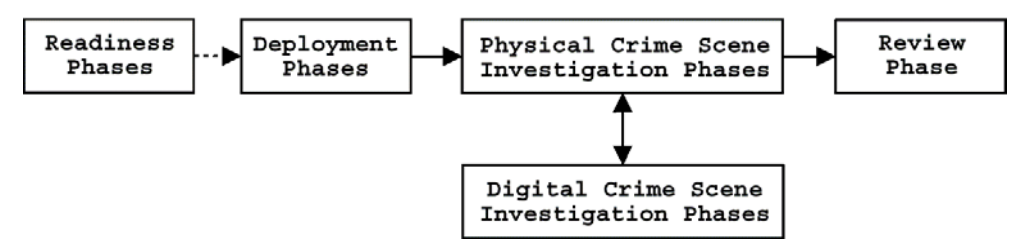
\includegraphics[width=0.8\textwidth]{images/IDIP.png}
  \caption{Integrated Digital Investigation Process Model (IDIP)}
  \label{fig:IDIP}
\end{figure}

Baryamureeba and Tushabe proposed a new model 
based on the best parts of the \gls{doj}'s \uline{Electronic Crime
Scene Investigation}, the \uline{Abstract Digital Forensics Model}, and 
the \gls{idip} model.  Their proposal was called the
Enhanced Integrated Digitial Investigation Process (EIDIP)\cite{baryamureeba2004enhanced}.
This model was proposed in 2004 at the annual Digital Forensic Research conference
(DFRWS)\cite{baryamureeba2004enhanced} and included the following phases:

\vspace{0.5 cm}
\begin{enumerate}
  \item {\em Readiness} -- same as \gls{idip}.
  \item {\em Deployment} -- which encompasses the Deployment,
  Physical Crime Scene Investigation, and Digital Crime Scene
  Investigation phases from \gls{idip}.
  \item {\em Traceback} -- that includes connecting the evidence collected
  in the previous phase to the suspect(s).  Typically this is done with \gls{ip}
  addresses and requires the authority to gather this information.
  \item {\em Dynamite} -- which includes the reconstruction of the events
  suggested by the evidence and the documentation and submission to the
  appropriate legal authories.
  \item {\em Review} -- same as \gls{idip}.
\end{enumerate}
\vspace{0.5 cm}

In 2006, Rogers et al proposed a reliable, repeatable process 
model designed specifically for digital evidence triage called
\gls{cfftpm}\cite{rogers2006computer}. It was created in partnership
with Purdue University's Cyber Forensics and Computer and Information
Technology Departments, along with the National White Collar Crime
Center. The process was derived from several other military and law enforcement models
including \gls{idip}, Digital Crime Scene Analysis (DCSA),
and a military Operations Order (OpOrd).  In coordination with the Southern Indiana 
Assistant U.S. Attorney's office and 
USADA Steve Debrota, Rogers et al implemented and reported
on the success of the \gls{cfftpm}\cite{rogers2006computer}.  This amalgamation of approaches is still inspiring 
the latest trends in Digital Forensic approaches.\\

Another researcher, Shaw et al, analyzed the Association of Chief Police Officers (ACPO)
and focused on the second step (Capture) as the primary guideline for evidential
integrity\cite{shaw2013practical}.  They strongly suggest compliance with
digital forensics best practices, like the ones provided in the ACPO.  Their final approach
and recommendation was to combine Linux utilities with a simplistic interface to standardize
the output and enable investigators who may not have full digitial forensic backgrounds
to perform triage on potential digital evidence.\\

The ACPO, a private company that helped establish and
develop policing practices in England, Wales, and Northern Ireland for many years,
put together a \uline{Good Practice Guide for Digital Evidence}\cite{williams2012acpo} in 2012 that outlines some
recommended procedures for dealing with digital evidence.  As with other methodologies, this guide
explains utilizing a four step approach: Plan, Capture, Analyze, Present.\\

The \gls{iso}/IEC 27037 guidelines (completed in 2012) provide an attempt at an internationally 
recognized approach,
with the goal of making it easier to compare, combine, and contrast
results for out-of-jurisdiction cases and for data scientists' research\cite{ISO27037}.  It provides a
common reference line for 
digital forensics\cite{ajijola2014review}.  But, it is not meant to replace laws or regulations.
The main purpose is to provide practical
assistance for investigations involving potential digital evidence, while preventing digital
evidence corruption.  This
process facilitates the usability of evidence by other jurisdictions.  This guideline provided
four steps for handling
potential digital evidence: Identification, Collection, Acquisition, and Preservation.  However,
this is incomplete, as
it only addresses gathering, not actually evaluating or providing results to law enforcement
investigators.\\

All of these different guidelines and approaches are intended to help find and gather digital evidence.
They are also intended to maintain the forensic integrity of the media devices.  Unfortunately, there 
is not a universally agreed upon approach. Some organizations combine these approaches
into a system of processes and procedures intended for use in their own facilities.  
Many organizations have home-grown solutions passed down from senior members of the digital forensics
team to the newer team members.  Not having a universally recognized and accepted standard 
leads to complications and difficulties when digital evidence needs to be shared across other
jurisdictions and boundaries\cite{ajijola2014review}.\\

The SEAKER device could be utilized to standardize an approach to the triage phase of 
digital media device investigation.  It is also easily altered to conform to an existing reporting
standard, if circumstances warrant it.\\

\subsubsection{Reactive Digital Forensic Investigation Processes}

\textit{Reactive} digital forensic investigation processes are utilized after an offense has been committed to help
identify the charges and suspects.  This is the most common process for digital forensics.\\

The SEAKER digital evidence triage tool is designed to help the reactive process.  
It is based on the reactive digital forensic investigation process with the goal of reducing the digital
forensic lab backlogs across the world in two ways.  The first way is to reduce the amount of digital
evidence acquired for the digital forensics lab.  This is done by enabling efficient and effective on-site triage to occur by
combining digital evidence collection and analysis into a single step.  The SEAKER device enables an initial 
collection of information and subsequent searches by any number of local,
on-scene investigators.  These investigators do not need extensive training in digital forensics to utilize it.\\

The second way SEAKER will reduce digital forensics backlogs is by enabling a faster, more streamlined approach to initial
potential evidence gathering and reporting.  This approach utilizes the SEAKER digital evidence triage tool to 
perform an initial acquisition and analysis on every existing case to provide a ``first-look'' at the information.
Within a few minutes of plugging in digital evidence media, SEAKER will enable digital 
forensic investigators a quick review of materials.  The process will help with prioritization of evidence, a basic
analysis and potentially initial evidence in the form of a report that can be provided to investigators and
prosecutors.\\

\subsubsection{Digital Evidence Triage}

Rogers et al (2006) seems to be among the first researchers to formally propose a
triage phase in digital forensic investigations\cite{rogers2006computer}.  The process 
(\gls{cfftpm}) is broken up into phases (see Figure~\ref{fig:CFFTPM}). 
The main phases consist of Planning, Triage, Usage/User
Profiles, Chronology/Timeline, Internet Activity, and Case-Specific Evidence.
Usage/User Profiles are broken down into three sub-phases: Home Directory, File
Properties, and Registry.  These are important and help distinguish user specific
activity and permissions.  The Internet Activity phase is also broken down into three
sub-phases: Browser Artifacts, Email Artifacts, and Instant Messenger Artifacts.
These also help establish user activity.  Some importance is explicitly stated to skip
based on type of investigation and prioritizing the investigation.\\

\begin{figure}[ht]
  \centering
    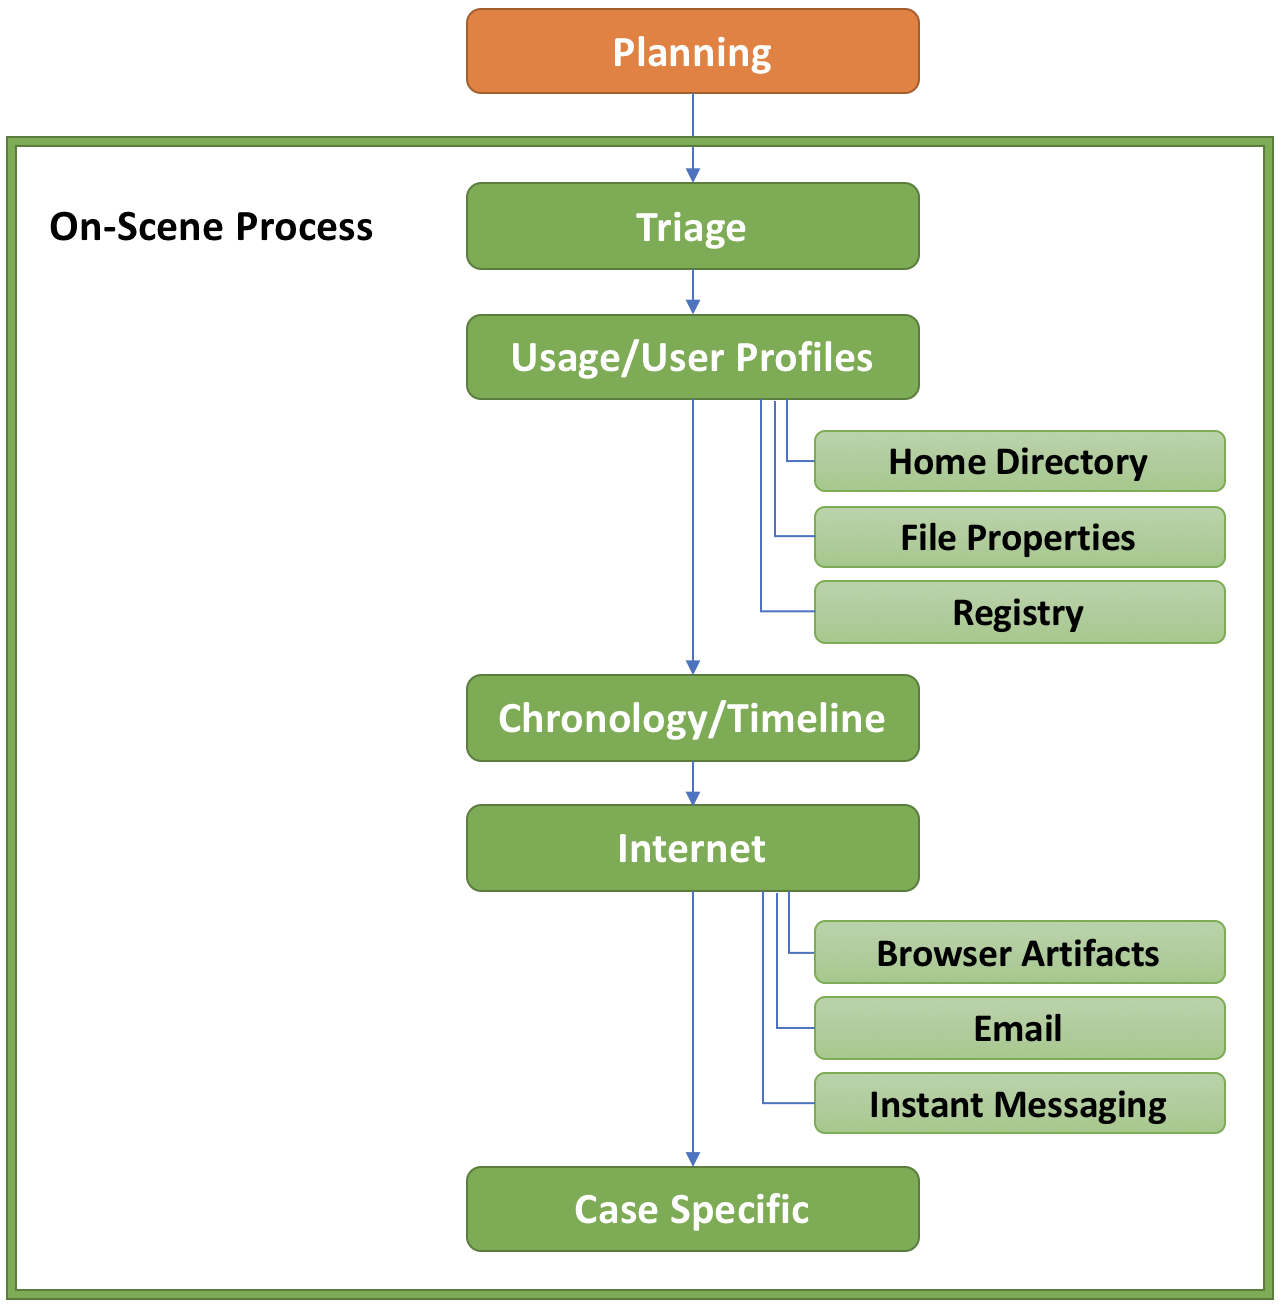
\includegraphics[width=0.8\textwidth]{images/CFFTPM.png}
  \caption{Computer Forensic Field Triage Process Model (CFFTPM)}
  \label{fig:CFFTPM}
\end{figure}

The process of triaging digital evidence is an especially effective method
when implemented on-scene at \gls{searchwarrant} execution time.  The \gls{cfftpm}  proposed
by Rogers et al was created to enhance the investigators ability to obtain
useful information at execution time of a warrant at the suspect's dwelling or place
of work\cite{rogers2006computer}.  The process is designed to be used in the first
few hours of the investigation, especially during the first suspect interview and
search execution phase of the investigation.  It is known that suspects are more
likely to divulge more information and be more cooperative in that environment
(Yeschke 2003\cite{yeschke2003art}).  As well, location of and presentation with
suspect ``triggers'' from the potential evidence increase the suspect's willingness
to talk and cooperate while on site\cite{rogers2006computer}.\\

The research done by Hitchcock et al also concludes that on-scene triage is
useful\cite{hitchcock2016tiered}.  They sought to expedite the process of
sending digital evidence for analysis and results.  One of their goals is to enable
more field triage of digital evidence to reduce the amount collected, and act
specifically on pertinent digital information.  They recommended that some
front-line crime scene investigators (non-forensic analysts) be trained in the
implementation of digital evidence triage and evaluation.  These trained individuals
would be DFT experts and have the ability perform field-level
digital evidence triage.  This triage would specifically weed out the benign from
the consequential digital evidence with high certainty, while also protecting the
digital evidence from spoilage and preserving evidentiary integrity.\\

Utilizing triage helps
reduce the potential backlog and associated delays in digital evidence gathering.
With the proliferation of \gls{iot} devices and cloud storage, the
field of digital forensics continues to expand.  These areas pose a great challenge,
but also new opportunities for investigative research and potential understanding
of cases.  Lillis et al researched cloud storage and found some areas of opportunity
to expand the digital forensics landscape, for instance parallel processing,
distibuted computing, GPU/FPGA utilization, and others\cite{lillis2016current}.
These areas for increasing the efficiency of ditigal forensics can be explored
further due to the substantially reduced I/O limitations in cloud storage.\\

Another potential augmentation to the digital evidence triage method was proposed by
Shaw et al and seeks to standardize on an approach they dubbed {\em enhanced
previewing}\cite{shaw2013practical}.  Enhanced previewing seeks to solve some of the problems
associated with typical triage approaches, but may fall short due to the extended time
necessary to complete the processing involved\cite{jusas2017methods}.\\

Shaw's et al enhanced previewing starts with an open source, CD-bootable image of
GNU/Linux and enhances its features to include boot-time application launching, and
a simple to use interface with minimal ability to deviate from task\cite{shaw2013practical}.
This bootable CD is intended to be placed into evidenciary computer
systems and booted using a series of BIOS modifications or boot-time interruptions.
This mechanism to boot the system off of a bootable CD is difficult, and where the
typical problems with untrained users of the enhanced previewing will happen.\\

This process of enhanced previewing does not take into account any \gls{iot} devices or 
cloud-based storage. It also assumes that there is a DVD drive or USB port available and
working, as well as the ability to access the computer's BIOS settings, as those
connections are not typically setup to boot by default.\\

As is the case in other research, Shaw et al extolls the need to reduce digital
forensic evidence analysis backlogs, especially with the evolution of big data and
the proliferation of digital devices\cite{shaw2013practical}.\\

The enhanced previewing concept has valuable merit, in that the collection mechanisms
are thorough.  Using the GNU/Linux based system and having written code for it, Shaw 
et al utilized some well thought-out approaches\cite{shaw2013practical}.  First, all
hard drives from the evidentiary system are mounted into the GNU/Linux filesystem as
read-only, thereby eliminating the need for write-blockers.  As well, the entire hard
drive is evaluated, including the file system, all partitions, unallocated space,
deleted files, and compressed files.  In addition, other mechanisms are employed that
continue to enhance the previewing are employed.\\

Shaw's et al proposal for a practical and robust enhanced previewing methodology aims to stem
the concerns of a typical triage process.  Risks still exist, for instance overlooking
digital evidence, but it is argued that those risks are outweighed by the risks of a
lengthy process due to large backlogs and the associated delays in evaluating that
evidence.  Another concern exists that inadequately trained people will be charged
with performing on-scene digital evidence triage and mishandling or incorrectly
evaluating results will cause evidence spoilage. Other concerns are the potential high
cost of software and training\cite{shaw2013practical}.\\

\subsubsection{Aquisition Methodology}

{\em Aquisition} has multiple definitions across the digital forensic universe.
Some define this as the process of gathering the digital devices, logging them using the 
{\em chain of custody} paperwork, and removing them from the location denoted in the
\gls{searchwarrant}.  Others define this as the collection of potential evidence from the digital
devices.  However, in this case it is meant to imply the entire set of processes and
procedures.  These include training the digital forensic examiners and SEAKER users, 
collecting the media that potential digital evidence may be stored on, and
gathering of potential evidence from each digital device.\\

The SEAKER tool is designed specifically for the triage phase of digital forensic
investigations.  As a general approach, this research will split the act of dealing with digital evidence into two
separate methodologies: {\em aquisition} and {\em analysis} (discussed in the next section).
These are the main foci since the SEAKER
device is designed to do both in a very timely fashion, with comprehensive searching results.\\

When a \gls{searchwarrant} is being executed, the SEAKER device is intended to be used to help
manage the triage process of the potential digital evidence.  This helps on-scene investigators
determine priority, potential to contain crime-related evidence, whether or not to seize the
device into custody, and documentation of the digital media\cite{hitchcock2016tiered}.\\ 

The set of processes and procedures for training and usage of the SEAKER device is well
documented in the appendix, but could also be supplemented by more specific guidelines that
combine the digital forensic lab's procedures with the usage documents.\\

The collection phase of aquisition specifically highlighted here is the gathering
of physical digital media information and the capturing of potential digital evidence content
in the triage environment.  The setup and training materials for creating and using the
SEAKER device are referenced in the appendix.\\

\subsubsection{Analysis Methodology}

Comprehensive forensic analysis of digital media is an arduous and time-consuming task.  A full
analysis could take many hours or even days and is not the first priority when serving a search
warrant.  The SEAKER device is intended to reduce the time this takes down to minutes,
especially during the triage stage of a \gls{searchwarrant} execution.\\

The {\em analysis} methodology is considered the second phase in the SEAKER approach and 
can consist of both the triage analysis stage and the full analysis stage.
Specifically, this research and the SEAKER device focus on the triage stage of Analysis.  This
stage can be applied in the field or at the digital forensics lab, while the full analysis
is unlikely to be accomplished in the field.\\

Digital evidence triage analysis is a very useful part of an investigation and can be 
implemented using the SEAKER device.  The triage analysis stage is considered in this research
to consist of an interactive web page that detectives and investigators can use to 
lookup search terms from the digital evidence collected from suspect devices plugged into the
SEAKER device.  It also consists of the reports that are generated and stored on the
SEAKER device.  The reports consist mainly of the metadata about the digital media and the
collection statistics, but does not include specific digital media content.\\

Previous versions of analysis included specific types of operating systems.
Rogers' et al research in 2006 covered the primary machine type at the time: the standard
Windows machine\cite{rogers2006computer}.  Unfortunately, focusing on a single operating system
leads to an outdated model over time, since the processes and procedures become obsolete as
new technology arises.  Along with the proliferation of \gls{iot} devices, new technologies
also have emerged as more mainstream that need to be incorporated into a more generalized
approach.  More operating systems are being utilized on a regular basis, like Linux, UNIX
versions, and Apple OS.  In fact, even our SEAKER device is an \gls{iot} device based on a
variant of Debian.\\

Other versions of analysis research deal directly with specific types of devices.
Ajijola et al reviewed the \gls{nist} guidelines that provide an in-depth
look into mobile devices, helping to explain the technology involved and its
relationship to the forensic process\cite{ajijola2014review}. This is useful, but not a complete analysis
guideline for law enforcement investigators.\\

The SEAKER device currently supports multiple operating systems, as well as multiple
device types (provided there is a way to adapt the device to \gls{usb}). It achieves the goal of
being device and operating system independent in terms of being able to collect content
information from digital media. The only limitation to the SEAKER device's ability
to read the content is the availablity of a device driver that allows mounting on Raspbian
Lite's operating system.\\

\subsubsection{Combined Aquisition and Analysis Methodologies}

The SEAKER project is intended to cover the areas of {\em aquisition} and {\em analysis}
with regards to the triage stage of an investigation.  In order to simplify the process and
enable non-digital evidence specialists to utilize the SEAKER device, both the
aquisition and analysis phases are combined.\\

In addition, the users are well guided along the path of aquisition.  Most of this process is
automated for ease of use and successful digital media content gathering.  The aquisition 
steps involved are:

\vspace{0.5 cm}
\begin{enumerate}
  \item Plug in the SEAKER device
  \item Wait 20-30 seconds
  \item Plug in the potential evidence via \gls{usb} to the SEAKER device
  \item Wait until the light stops flashing
\end{enumerate}
\vspace{0.5 cm}

The analysis side of the equation is also simple and well guided.  The user interface is 
designed to be very easy to use (see the Appendix section for exact usage details).  The steps
involved here are:

\vspace{0.5 cm}
\begin{enumerate}
  \item Connect to the SEAKER \gls{wifi} Access Point
  \item Bring up the webpage: {\tt http://seaker01.local}
  \item Choose which digital media devices to search
  \item \verb|Search| based on default or custom search criteria
  \item View results (expand/collapse tree-based format)
\end{enumerate}
\vspace{0.5 cm}

The combination of these two phases and the straightforward nature of the procedures to use
the SEAKER device make it an ideal digital forensics triage device.  The ability for
non-digitial forensic specialists to apply this technology is crucial to its feasability.
Hitchcock et al proposed and evaluated a ``tiered forensic
methodology'' model that defines a process of digital forensic triage utilizing non-digital
evidence specialists\cite{hitchcock2016tiered}.  They would be considered the first tier of
investigation and their
contributions are considered extremely helpful in the initial stages of a \gls{searchwarrant}.
The next tier is when the already-triaged digital evidence is sent for full evaluation from
a fully trained and qualified digital evidence specialist.
The potential evidence would be sent to a certified facility that can perform full digital
forensic analysis, called a \gls{tcu}.\\

This tiered approach is based on a Computer Forensic Field Triage Process Model proposed
by Rogers et al\cite{rogers2006computer} and the international standard \gls{iso} 27037
(Information Technology - Security Techniques - Guidelines for identification, collection,
aquisition, and presentation of digital evidence). The process model breaks down the six
phases of digital evidence categorization, which Hitchcock et al
loosely based their four phase approach on\cite{hitchcock2016tiered}.  The four phases are: planning, assessment,
reporting, and threshold.  The \gls{iso} 27037 standard specifically attempts to address the need
to minimize the risk of potential digital evidence being spoiled by mishandling, while also
attempting to maximize the evidentiary value of digital evidence collection.\\

Utilizing a tiered approach is not without risks.  One concern is the accidental exclusion
of an item of digital evidence that is important to the investigation.  Another is the
level of computer skills and training of the Digital Field Triage (DFT) expert.  An attempt
could be made to mitigate the latter with training and management process, while providing
evidence that the former is a common misconception in most cases\cite{rogers2006computer}.\\

Of course, the simplification of aquisition and analysis for use in a triage phase is also
not a full analysis. Certain factors related to recent advancement in technologies can cause
the SEAKER device to under-inform and potentially miss critical information.  One
example of missing potential evidence is when encrypted, compressed files or folders
are located\cite{shaw2013practical}.  Others include hidden or encrypted partitions,
password protected files and folders, images and videos obscured by significantly altering
the filenames and extensions, and use of rare, specialized operating systems. However,
these issues can all easily be overcome by marking the digital media as suspect and noting
it for review in the second tier at the lab.\\

This process cannot and does not supersede the ability or need to perform a full forensic
examination at a full-featured digital forensic lab\cite{rogers2006computer} or \gls{tcu}.  This
step is essential and necessary to fully consider all of the digital evidence that can
be obtained by full analysis.\\

Other research also indicates that combining the best pieces of process models and reviewing
latest digital forensic devices and methods are great ways to maintain adherence to 
good practices\cite{ajijola2014review}.  In 2014, Ajijola et al proposed a new process model
that is a hybrid of both \gls{nist} recommendations and \gls{iso} standards
with the resulting combination being much more effective than either of its individual
parts\cite{ajijola2014review}.\\

In the research for combining the \gls{nist} and \gls{iso} guidelines, Ajijola et al
explores the commonality, differences, and limitations of each model\cite{ajijola2014review}.  Although both models
follow the Auditability, Repeatability, Reproducibility, and Justifiability requirements, as
well as the Confidentiality, Integrity, and Availability standards, they individually lack some
necessary phases to enable them to be used separately.  The \gls{nist} process model lacks the
Identification and Collection phases, while the \gls{iso} process model lacks Examination, Analysis,
and Reporting aspects of a full Digital Evidence processing model.\\

The combination of these two approaches, as suggested by Ajijola et al,
provides a new five step approach: Identification, Collection and Acquisition, Preservation,
Examination and Analysis, and Reporting\cite{ajijola2014review}. These steps provide a more comprehensive approach that
law enforcement can use to fulfill its evidenciary duties in an investigation.  When both
process methods are used, the goals approach a full set of tasks from initial on-scene
evalutation to the end of the in-lab digital forensics investigation.\\

The combining of steps, approaches, and methodologies is encouraged.  The combination of 
aquisition and analysis works well in the SEAKER model because they are closely related,
function well as a pair, and encourage everyone to be able to use the tool for initial digital
media investigation.  The SEAKER
project combines the triage aquisition phase proposed here along with the analysis
phase, which is the rest of the \gls{cfftpm} on-scene process, into the full functionality
of the device.\\

\subsubsection{Digital Evidence Backlog}

Digital forensic labs and \glspl{tcu} are currently heavily inundated with cases needing
analysis and reporting of digital evidence.  To compound the problem, the amount of
data being created is growing astronomically.  The International Data Corporation
(IDC) forecasts that by 2025 the global datasphere will grow to 163ZB (see
Figure~\ref{fig:IOT}) (that is a trillion gigabytes)\cite{IDCDataAge2017}. That's ten times the 16.1ZB
of data generated in 2016. All this data will unlock unique user experiences and
a new world of business opportunities.\\

\begin{figure}[H]
  \centering
    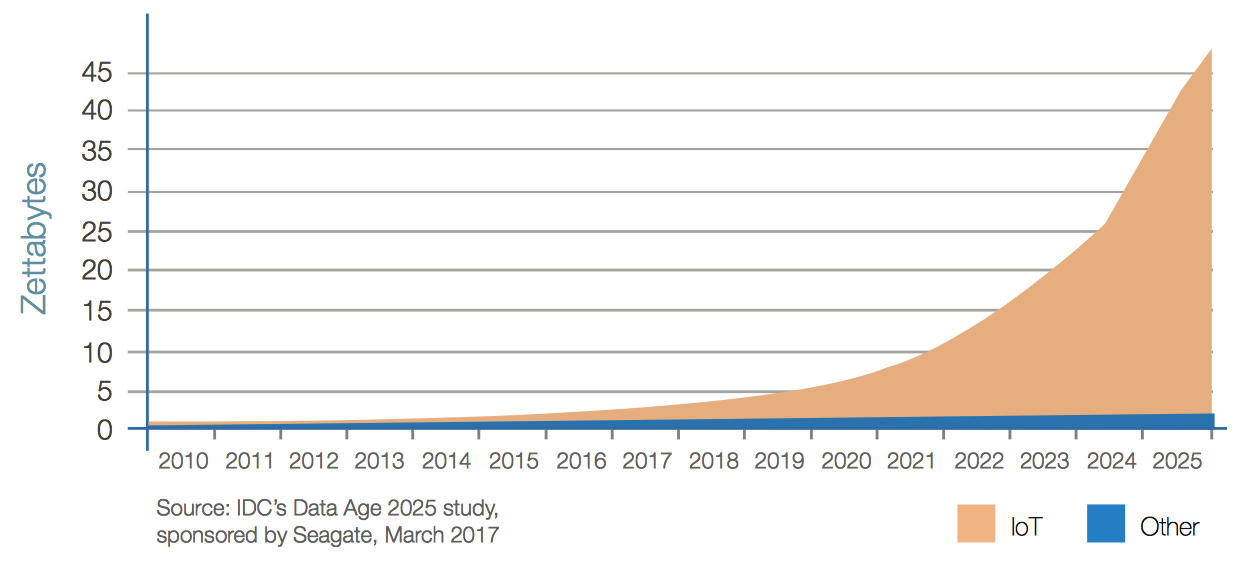
\includegraphics[width=\textwidth]{images/IOT_chart.jpg}
  \caption{IOT Device Data Growth}
  \label{fig:IOT}
\end{figure}

Some of the current challenges in digital forensic investigations are directly
related to the amount of data being created.  As Lillis et al
explores in their research, there are three main factors involved in the digital
forensic backlog: increasing number of devices seized per case, increased number of
cases involving digitial evidence, and the increasing volume of data per digital
media\cite{lillis2016current}.  This has lead to a growing and already substantial backlog in digital
forensic investigations.\\

As well, in Hitchcock's et al research\cite{hitchcock2016tiered}, they identified
a large and growing backlog of digital evidence.  They indicated that the extra
time required due to the backlog has led to problems in the law enforcement
community with regards to collecting, analyzing, reporting, and prosecuting.\\

Another effect of this increased delay and backlog is that cases become inactive,
waiting for new leads.  A more aggressive approach to solving the backlog could
help prevent dismissals, cold cases, and potentially more societal harm from a
potentially corrupt suspect of investigation.\\

Raghavan has accumulated a list of 5 major challenges
that the digital forensics community is facing and continue to add to the backlog
problem\cite{raghavan2013digital}.  The first is the complexity of binary data
aquisition, i.e. low level
data aquisition through digital media duplication.  This challenge causes the need
for sophisticated data reduction techniques.\\

Another complexity is the diversity of data and lack of standard examination
techniques.  The plethora of operating systems and file formats has been
increasing and is posing a more and more significant challenge over time.\\

The consistency and correlation problem is yet another challenge.  This is a
problem resulting from the current digital media investigation triage tools not
providing the entire picture to investigators.  Only part of the whole picture
is provided when these tools find digital evidence.\\

Another issue that Raghavan proposed is the volume of data to sort
through\cite{raghavan2013digital}.  The sheer amount of data that exists per user is increasing
at an alarming rate\cite{rogers2006computer}, and has lead to a very large backlog of digital
evidence to investigate.  These delays have even caused some cases to be dismissed.
This challenge is exacerbated by the lack of adequate automation for digesting the
data.\\

The last challenge proposed by Raghavanis the timeline synchronization issue with
digital evidence\cite{raghavan2013digital}.  Since the evidence could be
collected in different time zones, with different timestamp formats, clock skew,
etc., lining up the events in order can be challenging or infeasible.\\

These are all contributing factors, but some are reduced or eliminated when 
the digital evidence triage phase is implemented.  Even more issues are taken care
of when digital media devices are prioritized, excluded (due to lack of
evidentiary leads), and the digitial forensics backlog can be reduced.\\

The \gls{iot} also poses new challenges and could significantly
increase the backlog.  \gls{iot} devices are estimated to number near 40 billion by
2020, contributing to the overwhelming amount of digital data.  Since these devices
tend to have more non-persistent memory and less storage, this causes added
complexity for gathering and analysis.  This is a good case for expanding the 
potential uses of the SEAKER device to include more digital media devices.
In addition, a portion of \gls{iot} devices are battery operated and computationally
challenged, leading to loss of data over time, and the necessity of implementing
on-scene triage.\\

The backlog and delays in case reporting are contributing to a common problem of
time sensitivity\cite{hitchcock2016tiered}, especially related to being charged
with a crime and the legal process.  Some countries have given their citizens a
right to a ``speedy'' trial.  As well, some of the same countries have statutes
of limitation (limits on how long after the crime was committed to resolve the
case) for most crimes.  Some administrative situations are also contributors to
the backlog problem, for instance whether the case prioritization is based on
chronological filing, crime severity, or victim needs.\\

Everything that can be done to reduce or eliminate backlogs at digital forensic labs
or \glspl{tcu} should be fully utilized.  The SEAKER device is a great option for
many law enforcement organizations to begin that process.\\

\subsubsection{How SEAKER Can Help}

Instead
of attempting to put together an alternate operating system that uses the potentially
tainted computer system, the SEAKER device evaluates individual digital media
devices after being removed from the computer system it was originally from.  This
eliminates the possibility of self-deleting media, virus infection, and other 
potential hardware-related problems that may exist as evidence eliminating utilities.\\

The SEAKER device is portable in size, inexpensive to obtain (even in multiples),
simple to create and easy to use.  It is effective in on-scene triage, efficient in collecting and
searching digital media, and very well suited to handle the required purview of a digital
forensic device.\\

Digital forensics triage, especially with
the SEAKER device, has the opportunity to expand it's influence on the initial
investigation phase by expanding to incorporate digital evidence from
\gls{iot} and cloud storage devices.\\

The research of Hitchcock et al\cite{hitchcock2016tiered} should be referenced as a good
process starting point for new digital forensic labs.  As well, the SEAKER device is a 
great tools to enhance the existing law enforcement arsenal of digital forensic tools.\\

The SEAKER portable triage device can help by evaluating crucial
aspects of the file system and prevent the on-site investigators from skipping or
de-prioritizing critical potential evidence\cite{rogers2006computer}.  This is done by
collecting all of the filenames and locations of the entire media device and preparing
the SEAKER search mechanism.  The search mechanism is accessed via \gls{wifi} from 
investigator phones, tablets, or laptops.  Once connected to the SEAKER's \gls{wifi}
access point, the main webpage allows the media devices that have been 
attached to be selected and shows an editable, default list of keywords to search
for.  Once \verb|Search| is selected, the SEAKER device finds all matching keywords
from the filename and location list and returns any results found.  The results are
well formatted for browsing in an expandable tree-sectioned web page.\\

The SEAKER portable triage device can help eliminate some of the existing and
potential future problems that many jurisdictions face.  With shrinking budgets,
the lack of digital forensics specialists, coupled with the lack of technical prowess
of the on-site investigators and proper on-scene lab equipment\cite{rogers2006computer},
this new technology can easily and immediately benefit the law enforcement community.\\

\section{Background}
\label{sect-background}

In a labratory environment, digital forensics investigators have the ability to discover
a tremendous amount of material that is potential evidence.  This includes anything 
digitally stored on the evidentiary media from
explicity illegal files, to \gls{ip} address connections, to a digital chronology of
events.\cite{raghavan2013digital}\cite{rogers2006computer}
The software and hardware necessary to perform the
in-depth, full evaluation of the media are specialized for digital forensics 
work, but typically are costly, don't travel well, and can take many hours for
results from a single digital media device.\\

In the field environment, digital forensics
investigators are likely to not have the time, equipment, or proper environment to
obtain evidence from the digital devices found during the execution of a search
warrant.  In some cases, due to various reasons, digital forensics investigators
are not able to attend and therefore all of the digital media is taken into
custody for analysis at the digital forensics lab.  When they are able to attend,
they typically
bring a subset of their lab environment with them to start deciphering
the digital information and attempt to perform a triage analysis.\\

In a coordinated effort with the lead investigator at \gls{schttf} and his team,
this research is an attempt to help solve some of the field environment limitations
of digital forensics investigators.

\subsection{Legal Details}
In order for digital forensic investigators to obtain the data from a digital device,
a \gls{searchwarrant} for that device must be obtained.  As well, law enforcement must
obtain a \gls{searchwarrant} to acquire the device for searching in the first place.
Law enforcement must provide probable cause that a crime 
was committed and that items connected to that crime are likely to be found 
in the place specified by the warrant.  A judge will review the matter and if
they are in agreement, will authorize law enforcement to search a particular location
for specific items which are declared in the \gls{searchwarrant}.\\

After a digital device has been acquired by digital forensic investigators, they
must take special care not to alter the device's information in any way.  This 
requirement figuratively mimics the care a physical forensic investigator must
take to preserve physical evidence.  Special processes must be followed to ensure
that the potential digital evidence is not altered and, in fact, must be able to 
be proven if the matter ends up in a trial.  This is critical to ensure that the
evidence obtained from the device is admissible in court.\\

One device to aid in the proper handling of digital evidence is called a
write-blocker.  Digital forensic investigators use this device as an intermediary
between the devices and the computer systems they plug the devices into for
investigation.  The typical first step when a device is acquired by a digital
forensic lab is for the device to imaged (or copied bit by bit) so that the
image can be used for further evidence searching.  This provides an extra level of
abstraction, so that the actual device is kept in pristine digital condition.\\

Write-blocking has been implemented in digital forensics labs with an in-line 
piece of hardware.  Companies like Guidance Software and others have created
write-blocking devices that are added to the list of hardware necessary to 
prevent modification of any kind to the potential digital evidence.  The Tableau
product line is a great set of these types of devices.  Although they are made
to be simple and easy to use, they create yet another piece of the lab that must
be carried into the field and required to be plugged in and used.\\

For this research, the SEAKER device is intended to be used for triage investigation
on digital devices to perfom an initial search for potential digital evidence.
Instead of having a separate write-blocking device, the \gls{rpi} is set up with
write-blocking capabilities when digital devices are connected to it.  This
configuration enables the SEAKER's own system to act as a software-write-blocker
to prevent any digital alteration to the device.  This eliminates the need for 
the extra write-blocking device and reduces the footprint required to bring to
\gls{searchwarrant} exection.\\

\subsection{Technical Details}

Choosing the \gls{rpi} as the base platform for the SEAKER device was intentional
due to its low cost, extreme portability, and the ability to adapt it for use as
a digital forensic device.\\

\gls{rpi} is manufactured by the Raspberry Pi Foundation in the United Kingdom
for the purpose of teaching Computer Science in schools and around the world.  It
is a fully functional CPU with RAM, status lights, and input and output connections.
It has the ability
to be powered by batteries, \gls{usb}, or an electrical wall socket connection.
The form factor is small and the cost is kept to a minimum for ease of
aquisition, use, and adaptability.  As of this writing,
the most powerful version of the \gls{rpi} is \$35 USD.\\

The SEAKER device project is an example of how the \gls{rpi} device
can be converted into a working model.  Through the setup script, it is 
transformed into a fully featured digital evidence triage device.\\

A goal of the SEAKER project is to enable investigators without 
digitial evidence training and/or with limited computer training to utilize it
on-site at the execution of a \gls{searchwarrant}.  The SEAKER device is designed to
be self-sufficient and automatically self-preparing when it is plugged into a 
power source.  The device will boot, prepare the web server, the \gls{wifi} hotspot
and be enabled to handle digital devices that are attached to its \gls{usb} port.
Once a digital device is plugged in, it is automatically mounted and scanned.
A web-page interface was created for accessing the scanned devices when a portable
\gls{wifi}-enabled phone or tablet are connected to SEAKER.\\

These attempts to make the process as simple as possible are intentional and 
make the process of digital evidence triage aquisition and analysis
accessible to investigators with or without specialized computer knowledge or
training.\\

\section{Development of SEAKER Device}
\label{sect-developmentSeakerDevice}

The SEAKER device concept is very novel, not only in its capacity as a digital 
forensics evidence triage device, but also in the fact that it is low cost, highly
available, simple to setup and use, and provides very fast results.\\

There are other digital triage tools on the market, but almost every one is a
software solution that involves either a separate laptop or a bootable
CD, DVD or \gls{usb} drive to enable the interaction.  These types of software tools
typically require advanced computer knowledge and digital forensics specialists
to be involved.\\

Since the SEAKER device project was a collaboration with \gls{schttf}, it already has
built-in law enforcement acumen related to digital forensics.  The requirements were
provided the \gls{schttf} team.  They provided input during and after the development
of the initial prototype.  As a digital
forensics evidence triage device, it could be shaping the way investigators
handle computers and other digital equipment during execution of a \gls{searchwarrant}.\\

\subsection{Conception}

The proposal for the SEAKER device project initially came from the \gls{schttf}.  They wanted
a device that could quickly ascertain potential evidence and enable on-scene investigators
to search devices while questioning suspects.  This process of searching the digital devices
immediately is called triage.  With it, investigators are able to provide actionable
intelligence quickly, prioritize devices to be previewed, reduce preview setup time, and
triage larger amounts of devices.\\

The SEAKER device project specification was presented in the Masters level Cyber
Security class (COMP 524) at \gls{csuci} in the summer semester of 2017.  It was
proposed to the class by professor Dr. Michael Soltys during one of the initial
lectures as the final project for the course.  The attending students liked the idea
and work began on it immediately.
Dr. Soltys broke down the problem into categories so that student teams could form and
work on each piece individually.  The categories were:

\vspace{0.5 cm}
\begin{itemize}
  \item Connecting a digital media device to a \gls{rpi}, sensing OS and mounting (2 teams together)
  \item Searching in the mounted file system (2 teams together)
  \item Sending report to an iPad/laptop/handheld
  \item Documentation and troubleshooting
  \item Testing
\end{itemize}
\vspace{0.5 cm}

This breakdown helped guide each team to get started on their contribution to the
final project.  Before the students could begin, a few decisions needed to be made:
the device platform to use, the technology methods for input and output, and an
agreed on feature set.\\

The device platform chosen was the \gls{rpi}.  This enabled the students to work on the platform
independently, due to the inexpensive nature of it.  As well, two \glspl{rpi} were provided
for the classroom by \gls{schttf} and Dr. Soltys, respectively.\\

The input method chosen was setup for two types of input.  The first type was connecting
the digital devices to the SEAKER device.  This was agreed upon to be either with the \gls{usb}
port that was built into the \gls{rpi} or via a \gls{usb} to \gls{sata} converter cable.  This enabled
the digital device to be mounted by the Raspbian Operating System and automatically 
searched for content via the mounting rules.  The second type of input was human input
for a set of terms to search.  The search terms were agreed to be put into a web form that
would be submitted to the on-board web-server.\\

The output method clearly needed to match the input method in terms of technology, so the
use of the on-board web-server was chosen to be the output method.  When investigators are
using the SEAKER device, they would be shown a webpage asking them to submit a 
set of search criteria.  The results would be given back to the phone or tablet in HTML.
This also enabled the quick building of the HTML framework and response mechanisms.\\

Finally, the feature set needed to be agreed upon.  With direct guidance from the \gls{schttf},
specifically Frank Lyu, the class agreed to the following:

\vspace{0.5 cm}
\begin{itemize}
  \item Write-blocking of attached digital evidence devices
  \item \gls{sata} and \gls{usb} storage devices
  \item FAT, NTFS and EXT* file systems to be read from storage devices
  \item Filename-keyword filter
  \begin{itemize}
    \item Prepopulated keyword list
    \item Customization of keyword list
  \end{itemize}
  \item Status lights for power, and device status
  \item Wireless connection to a phone or tablet for keyword input and results
  \item Ability to find and display search results and digital device hardware information
\end{itemize}
\vspace{0.5 cm}

\subsection{Setup Script For Raspberry Pi}

The idea of a setup script for the \gls{rpi} was conceived by the author 
very quickly after the project was presented to the class, since
each team was assigned to work independently and the deadline of implementation was
extremely short.  In order to get everyone in
the class up and running and able to do work on their individual pieces, there
needed to be a baseline for everyone to start working with.  Starting with the 
base operating system image, called Raspbian, the setup script was meant to modify
it to handle the scenarios we were attempting to create.\\

First, there needed to be some initial setup for keyboard, timezone, \gls{ssh}, hostname,
and installing some additional packages.  To prevent unnecessary 
software from occupying the local Micro SD card, the ``Lite'' version of Raspbian
was chosen as the base operating system.  However, that meant that additional
Raspbian packages needed to be added; for instance, the Apache web server, a DHCP
server, PHP, the software to convert the wireless NIC card to an access point, and
the device drivers for FAT32, NTFS, HFS, EXT*, etc.\\

Next, the setup script needed to customize the SEAKER device based on user
parameters.  These include hostname, \gls{ip} address, DHCP supported range, the
default Raspbian user's (\verb|pi|) password, and the wireless access point password.\\

The setup script then prepares the \gls{rpi} access point configuration, web server
configuration, mounting rules, default web-pages, and compiles the custom C code
for searching (listed in appendix).\\

Finally, in order to avoid simple hacking and password locations, the setup
script clears the history, sets itself up to be deleted at boot time, and removes
any other reminants from the original setup.\\

Once the author finished programming the setup script to properly configuring the
device with a majority of the features, it was published to the class so that they could
begin using the \gls{rpi} as a SEAKER device and complete the minor bits of
functionality left.\\

\subsubsection{Web Server}

The author chose the Apache web server, since it is a standard Unix-based operating system
choice for serving web pages.  It also supports backend coding opportunities when 
coupled with a server-side code execution program like PHP.  Setting this up was
done by the author and was included as a part of the setup script.\\

A few steps were needed to implement the web server.  The first was to
load the Apache and PHP packages coinciding with the Raspbian operating system.  
Since it is a branch off of the Debian operating system, these were easily found and
worked well.  The next step was to load all of the files that were needed for
the HTML and PHP to display and operate properly.  The final step was to modify
the access to each of the files to be specifically accessible by the web
server daemon account.  This was necessary to ensure the files could be read and
served up by the web server when requested.\\

In addition, the {\em aquisition} code for searching the drive needed to have 
access to a shared location for the filename and folder searching algorithm.
The \textbackslash{}\verb|tmp| folder was chosen by the author as a suitable location, since
both the collection program and the web server have access to it.  An extra
feature of using \textbackslash{}\verb|tmp| is that the operating system clears
out the entire folder everytime it boots up, causing the previous data to no
longer show up.\\

\subsubsection{WIFI Setup}

The wireless NIC also needed to be setup to be a wireless access point so that
investigators could connect with a phone or tablet and use the web page access
to perform searches on the digital devices.  The main idea here was to have a 
password-protected closed network where the potential evidence could be searched.
This was included as a part of the setup script.\\

The steps involved here were complicated and difficult to setup properly.  As
with the web server, the proper Raspbian operating system packages needed to be
acquired and installed.  In addition, the setup of those packages required 
setting up DHCP, WPA, the wireless NIC, and the access point daemon.  Setting
these up mainly required adding and altering text configuration files.  
Unfortunately, researching the Internet was not much help, which lead to a
lot of trial and error testing by the author to make sure it all worked.\\

Finally, this process required a reboot, which was able to be postponed until
the end of the setup script.\\

\subsection{Rules For Mounting}

Mounting is the process by which the Raspbian Lite operating system attaches
a media device, providing access to the file system on that device.\\

During the setup script for the SEAKER device, auto-mounting is setup to
automatically mount new digital media devices that are plugged into the \gls{usb}
port.  Another script was written to handle the post-mounting {\em aquisition}
of the applicable drive contents.  The post-mounting script is also
configured to run once any new digital media devices are plugged in.\\

In order to accommodate the request to ensure the forensic integrity of the
suspected digital evidence, special mounting options were required.  There
are two different aspects for how drive contents can be modified.  The first is
the standard {\em writable} option, which allows the  files and folders to be
created, deleted, and modified.  The second is called {\em journaling},
which is an operating system concept for logging when and what the OS 
did to the drive.  Both options, \verb|ro| and \verb|noload|, are applied to
the mounting options.  This makes the SEAKER device functionally consistent
with a write-blocking device, as mentioned earlier in Chapter 2.\\

\subsection{Code for Searching Device}

The code for searching the digital devices was specifically aimed at gathering
every filename and location into a searchable file and storing it so that
those drive contents could be searched, even after the digital device had been
disconnected from the SEAKER device.\\

There were several options for searching for files.  The simplest way is to use
the built-in operating system mechanisms, for instance \verb|ls| or \verb|find|.
Another way is to code a simple C program that does the same thing.  There is
another built-in operating system mechanism that is much faster when used on
standard UNIX-based environments called \verb|locate|, however, that utilizes
an index that is built up over time and does not work well with newly
attached devices.\\

Since one of the goals of the SEAKER project was speed of collection, a test
was performed by the author that
measured the built-in mechanisms vs the simple C program.  The simple C program
was by far the fastest, beating the other two methods by an average of 26\%
(see Table~\ref{tab:CollectionAlgorithmData} for data).
The author's theory on why this is the case is that the other programs have many
built-in options and functionalities that are not utilized.  Those extra
functionalities have unnecessary code switches and therefore extra
execution paths that are not necessary for this file and directory collection
application.\\

\subsection{Web Code}

HTML and PHP were chosen as a simple interface for quick development.  It also
allows for easy access via many different devices through a standard web 
browser.\\

The main page (Figure~\ref{fig:MainPage}) was designed to be very easy to use
and as automatic as possible.
The list of searchable devices is populated at the load-time of the page.  As
well, the page refreshes itself until searchable media is found.  The 
default keyword search list is also shown on the page.  Each keyword is
searched independently and are entered one per line on the input keyword
text form.  The keyword search list is read in using
PHP from a pre-determined file that resides on the Micro SD card.\\

\begin{figure}[H]
  \begin{center}
  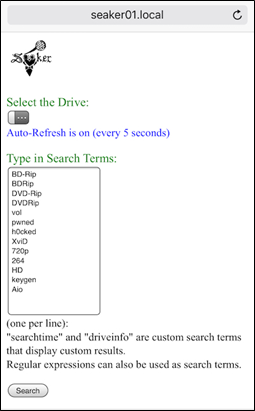
\includegraphics[width=6cm]{images/seaker-hh-screen-2.png}
  \caption{Main Page}
  \label{fig:MainPage}
  \end{center}
\end{figure}

When triggered using a \verb|Search| button, the media list and the
keyword list to search are passed to the web server via a webpage POST.  The
results page is then dynamically created using PHP to read each media's file
and directory list and write the matching results to the returned webpage.
The Raspbian operating system built-in command \verb|grep| is utilized to
find the results on the server side.\\

The resulting page (Figure~\ref{fig:ResultsPage}) is then displayed to the user 
using a simple HTML expand/collapse tool.  Each media searched and each search
criteria are accessible via this tree-like tool.\\

\begin{figure}[H]
  \begin{center}
  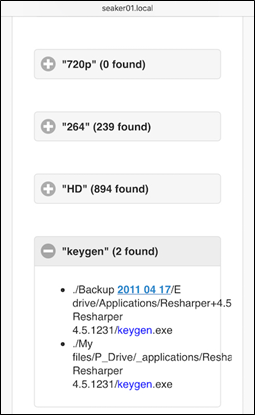
\includegraphics[width=6cm]{images/seaker-hh-screen-3.png}
  \caption{Results Page}
  \label{fig:ResultsPage}
  \end{center}
\end{figure}

In addition, some special keywords can also be used to obtain information
about the media.  The search term \verb|driveinfo| can be used to list the exact details of
the media, including serial number, size, and other information.
The search term \verb|searchtime| can also be used to show the time needed to find the
full drive information as well as the time for the particular search.\\

An administration page was also created for editing the default search keywords.
This page was intended to be password protected, but was instead conceiled by not
providing a link to it.  The full path to it ({\tt http://seaker01.local/keywords.php})
is required for access.  Once changed, the default search keywords remain permanently
altered for the SEAKER device.  See Figure~\ref{fig:DefaultKeywords}:\\

\begin{figure}[H]
  \begin{center}
  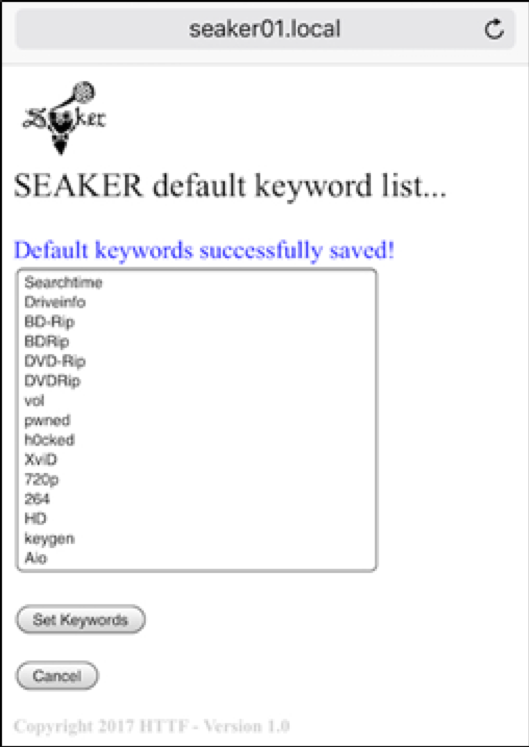
\includegraphics[width=6cm]{images/DefaultKeywords.png}
  \caption{Default Keywords page}
  \label{fig:DefaultKeywords}
  \end{center}
\end{figure}

\subsection{Process Flow}

The SEAKER device usage involves two main flows.  The first is the 
process of {\em aquisition}, which involves plugging it in to power
and then attaching digital media devices to it to be scanned.
The second process is {\em analysis}, as discussed in a
previous section.
See Figure~\ref{fig:ProcessFlow} for details.

\begin{figure}[H]
  \begin{center}
  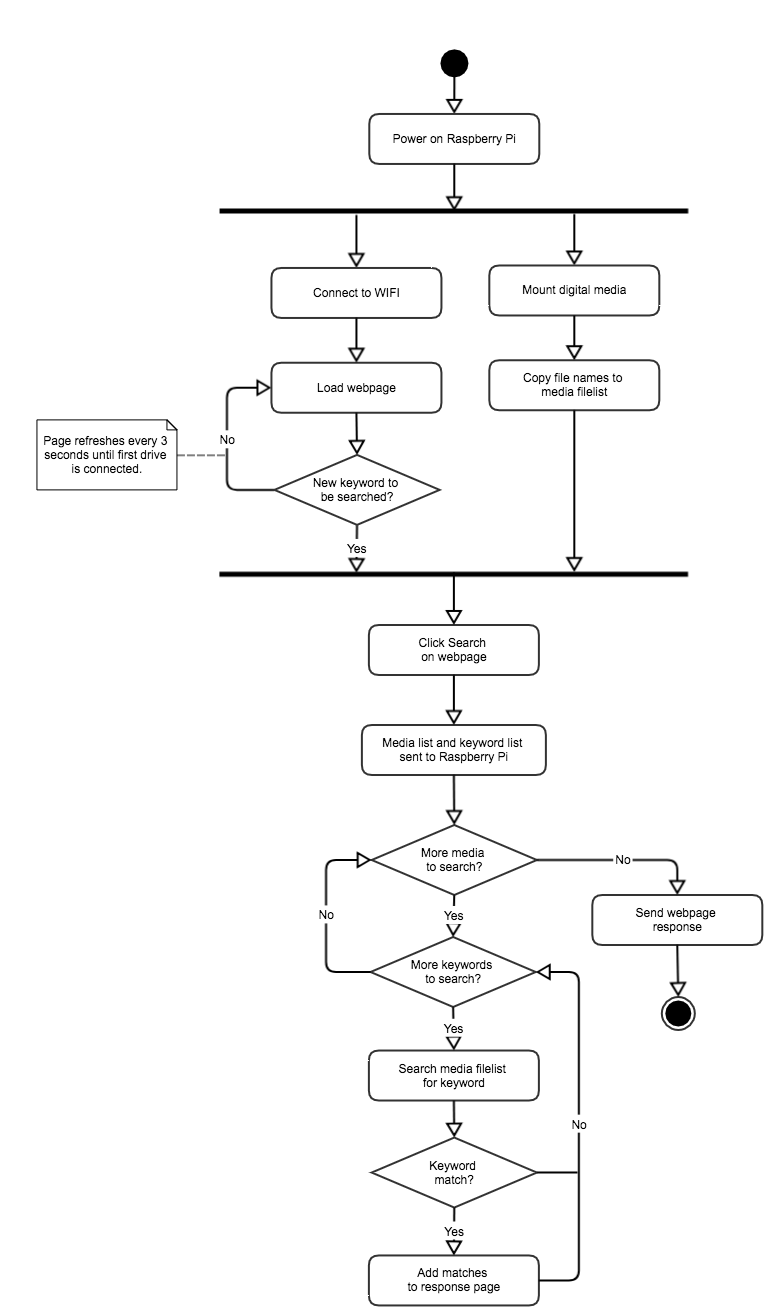
\includegraphics[width=11cm]{images/ProcessFlow.png}
  \caption{General Process Flow}
  \label{fig:ProcessFlow}
  \end{center}
\end{figure}

The process flow of SEAKER is a very simple design. After turning on
the Raspberry Pi, the two processes happen simultaneously. Immediately
when the drive(s) are connected to the Raspberry Pi, the file names
and their paths are collected and copied to a text file. Meanwhile,
the user must connect to the Raspberry Pi via \gls{wifi} on a separate
wireless-enabled device. The user must then open the SEAKER web page.
As shown in General Process Flow of Figure~\ref{fig:ProcessFlow},
the web page will refresh every 3 seconds, looking for new drives to
be connected to the Raspberry Pi. The first drive will be automatically added
to the list of drives available on the webpage to be searched. All
additional drives will appear in the list when the user refreshes
the page manually.\\

All user selected drives will then go through the search process as
shown in the lower section of the General Process Flow of
Figure~\ref{fig:ProcessFlow}. Each drive will be processed one at a
time. For example, the list of files for the drive will be scanned
for any matches to the first keyword in the list. The search is done
using the regular expression tool embedded in the Raspbian Linux
operating system called \verb|grep|. All files that are found to match
that keyword will be added to the output HTML. Once the entire file
list has been searched for that keyword, the process will begin again
with the next keyword in the list. This process will continue until
there are no more keywords to be searched. If multiple drives have
been selected to be searched, the same process will repeat itself
for each drive. Finally, the PHP engine will finish processing and
the HTML response page is finalized and sent back to the user's
mobile device.


\subsection{Tools Used for Development}

\subsubsection{Hardware}

(1)~{\em Raspberry Pi and power cord} - An affordable, very small
form-factor computer with average computing power. It is a powerful 
educational and research tool that follows the
standard ``von Neumann architecture'' by 
incorporating three main components: input/output devices, memory, and a 
central processing unit.  Models 3 and 3 B+ of the \gls{rpi} were used
for creation and testing of the SEAKER project. More information can be
found at {\tt http://raspberrypi.org}.

(2)~{\em Micro SD Card} - A solid state storage device that when combined
with a \gls{rpi} becomes a local hard drive for operating system, programs,
and storage while the SEAKER device is powered on.  The range of Micro SD
cards available are sorted by storage size and speed of reading and writing
(denoted by ``class'' designation).  For
the SEAKER device, the faster the write speed, the faster the
collection phase happens because of having to store the results.
A ``class 10'' or better cards have produced results more quickly than
other cards with slower write speeds.

(3)~{\em Powered \gls{usb} to \gls{sata} adaptor} - These devices are faily common, and
allow a \gls{sata} style hard drive to be connected to a computer through the
standard \gls{usb} port.  This enables \gls{sata} style hard drives to be connected
to the SEAKER device.  It is important to note that the \gls{usb} ports on the
\gls{rpi} do not have enough power to support powering larger hard
drives.

(4)~{\em Router or switch} - A router or switch allows multiple computers
to connect to each other using specialized software through network
interface cards.  During the setup phase of the SEAKER device,
one of these is necessary to be able to connect to \gls{rpi} with
another computer.  Remotely logging into the \gls{rpi} and running the
setup script is a required step (see setup steps in the appendix).

(5)~{\em Ethernet cable} - This is a hard-wire cable designed to connect
a computer to a network.  Since the setup process alters the wireless
network interface card, using the wireless interface of the \gls{rpi} to
connect to it is not an option for the SEAKER device.


\subsubsection{Programming Languages and Scripting}

(1)~{\em bash} - A UNIX-based shell, command language, and shell
scripting language used to gather and run a set of operating system
commands together.  Bash is used in several places in the SEAKER
project, including the setup script, as an auto-mount script
for automatic {\em aquisition} and in the PHP code to obtain and
push search details to the output HTML.

(2)~{\em c} - The c programming language is a mid-to-high level
language for writing computer programs.  This was used in two
locations to provide programs for media content collection
and for a late added feature to control a light-bar of LEDs that
plugs into the GPIO port of the \gls{rpi}.

(3)~{\em HTML} - A tag (or element) based system of organizing
information to be shown in a web browser.

(4)~{\em CSS} - An HTML styling language that simplifies the
ability to modify how HTML is displayed in modern web browsers.

(5)~{\em PHP} - A server-side programming langauge, typically
associated with dynamic web page creation.  For the SEAKER
project, this was a vital component of creating the search and
results web pages.

(6)~{\em JavaScript} - A client-side programming language that 
enables web developers to make web pages more interactive without
having to access server-side resources.

(7)~{\em JQuery} - A standard JavaScript library of useful
functions to simplify and expand the ability to make a web page
more interactive.

(8)~{\em Regular Expressions via grep} - Regular expressions are
a complex way to specify a search or replace pattern. A UNIX-based
operating system command-line utility, \verb|grep|, is
used to search for regular expression patterns in plain-text
files.  This is a very critical part of the SEAKER device, since
the searching mechanism plays a vital role in the project.

\subsubsection {Raspbian Operating System}

(1)~{\em Raspbian Linux (a Debian distro)} - One of the standard
operating systems that support the \gls{rpi} hardware.  It is
derived from the Debian operating system.  There are two versions
available for every release: Full and Lite.  The full version
provides lots of useful default packages, a built-in user interface
and a very simple to use guided setup.  The Lite version provides
only a minimum of packages, no built-in user interface (with the
exception of a command line), and no initial guided setup.  In
order to keep the SEAKER project as uncomplicated as possible, 
the Lite version of the Raspbian operating system was chosen.

(2)~{\em grep} - A command-line utility included
with almost every UNIX-based operating system.  It is widely
known as a very powerful tool for finding regular expression
patterns in plain-text files.  In the Raspbian operating system,
the initial configuration contains some useful features that
colorize the results of \verb|grep|.  Unfortunately, this also slows
down the \verb|grep| mechanism due to the extra code burden.  The
SEAKER setup script removes the color features of \verb|grep| to 
enable the fastest searching experience.  It also changes the
default searching mechanism to ASCII search,
enabling an even faster \verb|grep| result.

(3)~{\em apt-get for Raspbian packages} - Advanced Packaging Tool
packages are automatically searched, downloaded, and installed
using the apt-get command-line utility.  It is a tool based
on the Debian software packaging system.  The SEAKER project
uses this tool inside the setup script to add necessary
packages to the Raspbian Lite operating system.

(4)~{\em Apache HTTP server} - An industry standard web
server application that is open source and cross platform.

(5)~{\em PHP add-on for Apache} - Hypertext Preprocessor utility
that enables a programming language for server-side coding.

(6)~{\em Rules file for auto-mounting} - The {\em udev} utility 
is a userspace device manager for Linux-based operating systems. 
One mechanism of device control is to write a simple script file
called a ``rules'' file
(similar to a shell script) that enables the device manager
to automatically control the specified device(s).  Because 
the SEAKER project is intended to auto-mount digital media and
launch a collection script to gather the information
from it, a rules file was created during the setup script
that enables the device manager to automatically perform
these tasks.

\subsubsection{Collaboration Tools}

(1)~{\em Gliffy} - A free Google Chrome application that enables the diagramming
of charts, graphs, flowcharts, and other drawing templates.  This tool
has a simple drag and drop interface that allows for online collaboration 
and sharing during diagram creation.  The SEAKER project participants
utilized this for creating flowcharts describing the user and process
flows.

(2)~{\em Slack} - An online instant messaging and group chatting platform
freely available for simple use.  The SEAKER project participants utilized
this for collaborating, setting up meetings, online video discussions, and
some initial document sharing.

(3)~{\em AWS S3} - Amazon Web Services' Simple Storage Service (S3) is for online
storage of files.  The SEAKER project utilized this for beta versions of
the setup script and eventually storage of the final working version along
with the documentation to accompany it.

(4)~{\em GitHub} - An online code sharing, repository, and version control
system.  It is widely known to host many open source projects and repositories.
The SEAKER project used it during development to share the code base and
create an informational readme file that is displayed in {\em GitHub} on
the main repository page.

(5)~{\em Dropbox Paper} - An online document repository and collaboration
tool that enables multiple people to edit the same document simultaneously.
The SEAKER project team utilized this tool for writing up the setup guide, 
user guide, technical specification, and presentations.

\subsubsection{Setup Tools}

(1)~{\em Hardwire Connection to the Internet} - The SEAKER setup script
requires a connection to the internet in order to download the necessary
operating system packages.  The ideal SEAKER setup environment is to 
connect the \gls{rpi} to a router or switch that is also connected to 
the internet without a proxy server.  This allows another computer to
securely connect to it as well as having a connection to the Internet.

(2)~{\em Apple Computer System: Etcher, Paragon NTFS, terminal, \gls{ssh}} - If the
secondary computer required to remotely access the \gls{rpi} in order to run the
setup script is an Apple computer, a program like {\em Etcher} will load
the initial Raspbian Lite operating system onto the Micro SD card.  It is a
tool for copying a disk image from an image file to a 
Micro SD card.  Another tool is an NTFS reader/writer driver like {\em Paragon
NTFS}.  It is necessary in order to access the newly copied image of Raspbian Lite
on the Micro SD Card.
This is used to copy the setup script and enable \gls{ssh} access to the \gls{rpi}.
Finally, a command line program like {\em terminal} can be used to remotely and
securely connect to the \gls{rpi} after the Micro SD card is installed and the 
system is booted.

(3)~{\em Windows Computer System: Win32DiskImager, Windows Explorer, Putty} - 
If the secondary computer required to remotely access the \gls{rpi} in order to run the
setup script is a Windows computer, a program like {\em Win32DiskImager} is used to load
the initial Raspbian Lite operating system onto the Micro SD card.  It is a tool
for copying a disk image from a file onto a Micro SD card.
Another required action is to access the newly copied image of
Raspbian Lite on the Micro SD Card. This is necessary to copy the setup script
and enable \gls{ssh} access to the \gls{rpi}.
Finally, a \gls{ssh} program like {\em Putty} can be used to remotely and
securely connect to the \gls{rpi} after the Micro SD card is installed and the 
system is booted.


\section{Experimental Results}
\label{sect-experimentalResults}

\subsection{Prototype Demonstration}

As the final project in the summer 2017 Cyber Security class, the SEAKER device
project was presented to the \gls{schttf} representatives and other faculty and
administration from \gls{csuci}.\\

The SEAKER device presentation consisted of an introduction from Dr. Soltys, a 
slide presentation from every student team, and a recommendation for hardware to 
use for real-world SEAKER implementations.  It also included a live demonstration
of SEAKER's functionalities with digital media provided by the \gls{schttf}.
In advance, \gls{schttf} prepared one external hard drive and two USB thumb drives
for the class to collect files on in real-time during the presentation.  These
devices had not been seen by the students prior to the demonstration.\\

The live demonstration was intended to be fully
functional and prove that a prototype could be created using the described
parameters and features requested.  In addition to the three devices \gls{schttf}
provided, the audience was also encouraged to participate
as ``detectives'' using their personal phones to experience the SEAKER functionality
first hand.  An Apple iPad was also used by the presenters to participate as
``detectives'' and had the experience projected on a screen for the audience.
This allowed everyone to see the SEAKER working in real-time.\\

The demonstration began with an initial test using a hard drive that had previously
been tested and found to be able to be acquired and analyzed.  After attaching it
to the SEAKER device, the auto-mount script ran automatically and the information
was properly collected and searchable.  The auto-refresh functionality on the
webpage worked as expected and showed the attached media as a selectable drive.
A quick search also was successful and the product was demonstrated without flaw.\\

The \gls{schttf} prepared digital media devices were tested next.  All three devices
were able to be auto-mounted, collected, and searched.  \gls{schttf} then provided
search criteria after the drive information was collected.  The final phase was to perform the
search and see if the proper fileset was exposed in the results.  The conclusion
of the live demonstration was that the fileset was properly found and the SEAKER
device was properly working and ready to experiment more in a real-world situation.\\

SEAKER also proved very successful as a WIFI access point to the ``detectives'' in
the audience.  Multiple different phones were used to connect and search.  All were
successful in utilizing the SEAKER, as well as the iPad used in the demonstration. 

\subsection{Results}

TODO:\\

graph of latency\\

estimates of time vs data Gb\\

examples of running on Frank disks\\

\section{Conclusions and Future Work}
\label{sect-conclusionAndFutureWork}

The SEAKER device was successfully created with the agreed upon functionality.  It
properly acquires digital media content and enables analysis by investigators
via \gls{wifi} connections to the \gls{rpi}.  It collects potential digital
evidence without the fear of tainting the evidenciary integrity.  And, it keeps a
log of devices that have been aquired.\\

It shows promise for real world law enforcement via digital forensics triage.  The
SEAKER device is useful for on-scene investigations during search warrant
execution.  It is also useful for helping reduce the backlogs at digital
forensics labs.\\

The SEAKER project was a successful collaboration between two different institutions in the public
sector: law enforcement and academia. The former has many interesting problems to offer, but as they
are overwhelmed with cases they typically do not have the man power to do research and development.
The latter is happy to do the research and development, as it enhances the educational experience of the students to be learning
in the context of applications to real life problems. It is a fortuitous and symbiotic relationship, and we
plan to embark on other such projects in the future.\\

SEAKER is also the testament to the fact that supremely useful devices, meeting the needs of
practitioners, can be constructed from relatively simple components; what is required is expertise and
enthusiasm, which in the best cases academia possesses in ample measure. \glspl{rpi} are a revolution in
embedded controllers, and we are just scratching the surface of their applicability. They are inexpensive,
but wield the power of the Linux Operating System.\\

The potential uses for the SEAKER device are great with the existing set of
functionality.  More so, the future potential functionalities are even greater.\\

The general implementation and code do have some limitations.  For instance,
in addition to the regular expressions, there could also be fuzzy matching, size
grouping, internet browser data, registry, swap file, and email searching, and
many others.  These improvements may be implemented by future students, or by digital
forensics professionals. We encourage anyone who implements them to share their work; the main bash
script for the SEAKER device is available on github at {\tt https://github.com/michaelsoltys/seaker}.\\

The SEAKER device only supports a few filesystems, whose contents can be collected
(namely, NTFS and FAT (exfat, FAT32, FAT16...)). There may be unknown bugs to be worked out
in the supported filesystems, and there is certainly work to be done in expanding the
list of supported systems.\\

If an unsupported filesystem is found on the digital media, it may fail to
mount and not show up on the SEAKER's search page at all. Similarly, digital
media that cannot be read or are not supported do not appear; the search page
displays them only after files have been collected. Here, there is opportunity
for improvement: as opposed to displaying digital media for which collection is
complete, SEAKER could display all devices attempted with a status next to each. This
status could be one of three states: failed search,
collection in progress, and collection complete.\\

It can be difficult to match a hard drive to its corresponding search results. Partitions are uniquely
identified by a UUID, and some properties (capacity, for example) are displayed with the search results,
but these properties do not provide a perfect way to determine which physical device corresponds to
which mounted partition or device. Storage devices generally have a serial number of sorts, but this
serial number is not visible to SEAKER. This is a problem which requires some creativity to fully solve.\\

SEAKER could also take a picture when a drive is plugged in, and associate that picture with the search
results, for instance, but this solution requires that investigators position each storage device in front of
a camera; this approach requires a camera, and moreover it is tedious and error-prone.\\

When a search finds a hit (i.e., a matched expression or file extension), investigators may want to
view the corresponding file. As SEAKER is currently set up, this would require them to manually find and open the file. Speed
and ease of use are priorities, so it would be best if investigators could select a file in the search results
and have SEAKER fetch a copy of it for them. This function inevitably requires that the storage device
being queried is still connected, assuming that this condition is met, copying and viewing a file should
not be too complex.\\

Similarly, it would be useful if investigators could view thumbnails of images and videos in the search
results. One example of the motivation here is child pornography cases; incriminating images may have
innocuous names, but thumbnails would indicated the true content.\\

This leads to another issue: as incriminating files may be named innocuously, investigators will often
want to search simply for all images, videos, etc. SEAKER could minimize the work necessary by
allowing for preset groups of search terms, which can be created and edited by administrators. For
example, an admin could create an ``images'' group which causes SEAKER to include jpg, pdf, png...\\

We are very interested in a ``Data Carving'' option. Data carving is the identification and extraction
of files from unallocated clusters using file signatures. A file signature, also commonly referred to as a
magic number, is a constant numerical or text value used to identify a file format. The object of carving
is to identify and extract (carve) the file based on this signature information alone. We are interested in
hidden files (which are sometimes easy to locate, as for example in UNIX with \verb|ls -a| command) and
deleted files, which is more tricky as the files can be partially overwritten. A partially overwritten file may
still constitute valuable evidence: for example, a portion of an image can be taken as solid evidence that
the entire image was on the disk at some point. How can one establish whether a portion of an image
comes from a particular image? It seems that the only way to accomplish that is by visual inspection,
and having an investigator recognize the original image. In order to automate this process one could
attempt one of two things: build a massive database of frequently circulating (say, CP) images, and
hashing different formats of these images (.pdf, .jpg, .giff, .tiff, etc.), as well as different resolutions,
and chunks of standard sizes (say, 64Kb). This still seems like a shot in the dark. The second approach
is to define something akin to fuzzy hashes, the type of hashes that are used to recognize variants of the
same malware. This new type of fuzzy hashing would be invariant under differingb formats, or standard
resolutions, and chunks of an image could be identified by close proximity to the original hash. Hits
would be still confirmed visually to avoid false positives; a bigger issue would be false negatives.\\

Finally, documentation is important in any investigation. When triage reveals media which motivates
investigators to confiscate the corresponding storage device, they should document this motivation. As
such, it would aid investigators if SEAKER could generate a search report for a selected drive from
the search results screen. This report could be downloaded to the investigator’s device or saved on the
SEAKER unit for later access by an administrator. It should contain the search results along with some
circumstantial information, such as the date, the name(s) of investigator(s) requesting the report, and
their reason for confiscating the device.\\

Another potential area for improvements to existing code could be a location for
entering passwords obtained from suspects.  These could be used to unlock entire
drives, zip files, PDFs, user folders, files, email, website usage, etc.  This
could also be extended to find online account passwords, especially in the case
of browsers that allow saving site-specific usernames and passwords.\\

The \gls{schttf} has asked for some new functionality as well.  They would like the
ability to search multiple partitions, local \gls{wifi} networks and access levels, 
thumbnails of images and videos, support newer operating systems (APFS and
HFS Plus), and extract \gls{ip} addresses from known suspect configuration files and 
other locations.  These are just a few of the requests, but seemed to be at
the top of their list.\\

There are also many different libraries that could be included and built
into a searching algorithm.  Be aware that these will slow down the gathering
process and could be more useful if searched in stages.  Here are a few:

\vspace{0.5 cm}
\begin{itemize}
  \item LibForensics -- {\tt http://code.google.com/p/libforensics/}
  \item Volatile Memory search -- (Volatility: {\tt http://code.google.com/p/volatility/}) and (WindowsSCOPE: {\tt http://www.windowsscope.com/})
  \item Oxygen for mobile -- {\tt http://www.oxygen-forensic.com/en/features}
\end{itemize}
\vspace{0.5 cm}

In researching this topic a lot of other potential improvement features
came to mind.  This is by no means a comprehensive list, but it is a start:

\footnotesize{
\vspace{0.5 cm}
\begin{itemize}
  \item More supported media types
  \item Add AJAX (or similar technology) to give live feedback for search and collection
  \item Create RESTful API for using Raspberry Pi
  \item Clean up HTML code, use CSS
  \item Write SEAKER iPhone/iPad/Android apps to connect to Raspberry Pi and perform searches, edit keywords, etc.
  \item Use heap memory instead of stack memory for path
  \item Better way to skip . and .. (possibly always skip first two directory entries?)
  \item Reduce size of file/directory listing file. This may involve changing how to \verb|grep| or implementing custom \verb|grep|
  \item Possibly store files in a database instead of a file
  \item Implement the ability to connect to Raspberry Pi using Bluetooth instead of \gls{wifi}
  \item Customize web pages for device type
  \item Use a better wireless network adapter for better range. These adapters are inexpensive.
  \item Implement Linux setup with puppet/cfengine/salt/etc.
  \item Better error messages about why drive could not be read
  \item Add a “Blinkt!” light panel to show visual status of the Raspberry Pi
  \item Check the health (SMART status) of the hard drive before scanning
  \item Add support for RAID, mSATA, SCSI hard drives (\verb|mdadm| is a RAID driver for Unix-based systems)
  \item Read directly from rawdisk to find file list to speed up collect
  \item Make SEAKER an available Raspbian/Debian package
  \item Support unicode filenames
  \item Auto-unmount the hard drive at the end of collection
  \item Support multiple partitions gracefully
  \item Search for filename matches only
  \item Search for path matches only
  \item Offer option via checkbox for searching inside compressed files
  \item Offer option via checkbox for searching inside text files
  \item Find all deleted files (foremost, ntfsundelete)
  \item Search deleted partitions and unpartitioned space
  \item Build another web page for troubleshooting/access/administration/etc.
  \item Search on-media virtual hard drives (vhd, vdi, vmdk) (vmware, virtual pc, parallels, hyper-v)
  \item Search on-media hard drive images (.iso)
  \item Searching the raw drive instead of using the on-media operating system
  \item Online hard drive investigation (i.e. Cloud Forensics)
  \item Network Traffic Investigation
  \item Video segmentation and video image hashing
  \item Crime-specific searchs:
  \begin{itemize}
    \item financial crimes
    \item credit card fraud
    \item hacking
    \item bullying
    \item blackmail
    \item espionage
    \item fraud
    \item customizable (corporate / military)
  \end{itemize}
  \item OS lockdown (raspbian)
  \item Decrypting encrypted devices (password entry location, assessment without password)
  \item Utilize forensics as a service
  \item Integrate with Microsoft's photoDNA cloud service
  \item Build an iPad app to provide simpler, more guided use
  \item Query Expansion - automatically searching for same query maybe in other contexts
  \item Synonym Matching - automatically searching for similar words to the query word
  \item Collect everything in UTC time for chronology matching
  \item Universal way of collecting hard drive hash value for verification of evidence integrity
  \item Data Visualizations:
  \begin{itemize}
    \item present all data visualizations for a particular drive or all hard drives
    \item graph - size vs amount of files (one hard drive, and all hard drives)
    \item graph - common details (like file type, etc.) maybe make it clickable!
    \item graph/chart - files by date
    \item graph/chart - files by file type
    \item chart - website visits
    \item digital image hashes list (stored and compared)
    \item many others...
  \end{itemize}
  \item Improve analysis speed: skip known OS files, known applications files, etc.
  \item Investigation Gathering rollup: (possibly stored online or in a report)
  \begin{itemize}
    \item Database schema for storing case specific data
    \item metadata
    \item Unique ``gathering ID''
    \item case number
    \item observation report
    \item crimes severity
    \item potential offenses
    \item time gathered
    \item gatherer
    \item suspect list
    \item location gathered
    \item suggestions for other research
    \item which computer system it came from
    \item Set of evidence
    \item Digital Evidence item
    \item images of item
    \item unique item ID
    \item file contents
    \item ranking within set of evidence
    \item image thumbnails
    \item collection statistics
  \end{itemize}
  \item Find encryption Keys 
  \item Thumb strips of videos
  \item Predetermined search criteria (passwords, pw, etc.)
  \item Output more file information: file owner, MAC times
  \item Sorting ability, for instance make it based on user or access times
  \item Ability to search by time, i.e. time=lastweek, time=5/5/18-5/15/18
  \item Internet usage timeline
  \item Auto-search / Auto-filter
  \item For drug related crimes, search... Spreadsheets, documents, databases, internet purchase strives
  \item For financial related crimes, search... Spreadsheets, databases, MSMoney, Quicken
  \item CRC of any acquired files (for later integrity comparison)
\end{itemize}
\vspace{0.5 cm}
}

For the students, the experience was invaluable. Perhaps the most important aspect was non-technical:
how to work well in a large team. There were eighteen students in the class; a composition of different
backgrounds, talents and strengths.\\

Digital forensics and academia would both benefit greatly from increased collaboration; students can
offer relatively inexpensive development in exchange for real-world experience and the opportunity to
create something which will be used. As a side effect more students would consider digital forensics
as a career, resulting in some level of alleviation of the problems mentioned in the second quote in the
introduction\cite{hitchcock2016tiered}.


\section{Appendix}
\label{sect-Appendix}

\subsection{SEAKER Setup}
The following set of instructions will detail how to setup the SEAKER
environment for the first time. There are three install options that
enable SEAKER creators to prepare the device.  See
Table~\ref{tab:RequiredSoftware}

\vspace{0.5 cm}
\begin{enumerate}
  \item {\em Router} -- This option is where the \gls{rpi} and the
  secondary computer are connected directly to the same router, thus
  allowing the same local DHCP to assign the IPs of both.  The
  secondary computer is used to prepare the Micro SD card and to later
  remotely and securely connect to the \gls{rpi} to complete the
  setup.
  
  \item {\em Direct Connect} -- This option is where the Raspeberry Pi
  is connected directly to a monitor and keyboard to enable direct
  user input via the termnial.  The secondary computer is necessary to
  prepare the Micro SD card, but not used to remotely connect to the
  \gls{rpi} to complete the set up.

  \item {\em Corporate LAN} -- This option is almost identical to the
  {\em Router} option, but utilizes a corporate network instead of
  a local router to connect to the \gls{rpi}.  This option is the
  most IT intensive, since the \gls{ip} address assigned to the Raspberry
  Pi is often not easily found.
\end{enumerate}
\vspace{0.5 cm}

\begin{center}
  \begin{tabular}{l|l|l}\hline\hline
    {\bf Option 1}    & {\bf Option 2}         & {\bf Option 3} \\
    {\bf (Router)}    & {\bf (Direct Connect)} & {\bf (Corporate LAN)} \\\hline\hline
    \multicolumn{3}{c}{}\\
    \multicolumn{3}{c}{Hardware Required} \\
    \multicolumn{3}{c}{}\\\hline
    & & \\
    \textbullet \gls{rpi} & \textbullet \gls{rpi} & \textbullet \gls{rpi} \\
    \textbullet Mac or Windows Computer & \textbullet Mac or Windows Computer & \textbullet Mac or Windows Computer\\
    \textbullet Micro SD card & \textbullet Micro SD card & \textbullet Micro SD card\\
    \textbullet Router & \textbullet Monitor\\
    & \textbullet Keyboard\\
    & & \\\hline
    \multicolumn{3}{c}{}\\
    \multicolumn{3}{c}{Software Required} \\
    \multicolumn{3}{c}{}\\\hline
    & & \\
    \textbullet Raspian Stretch Lite & \textbullet Raspian Stretch Lite & \textbullet Raspian Stretch Lite \\
    \textbullet \gls{ssh} client & \textbullet \gls{ssh} client & \textbullet \gls{ssh} client\\
    \textbullet Disk Imaging software & \textbullet Disk Imaging software & \textbullet Disk Imaging software\\
    \textbullet \gls{ip} Scanning software & & \\
    & & \\\hline
  \end{tabular}
  \captionof{table}{SEAKER set up: Required Hardware and Software}
  \label{tab:RequiredSoftware}
\end{center}

The following creation process is required to setup the SEAKER device
to the specifications outlined in this paper.  Figure~\ref{fig:SeakerCreation} 
outlines the general process, while the specific steps are listed below.

\begin{figure}[ht]
  \begin{center}
  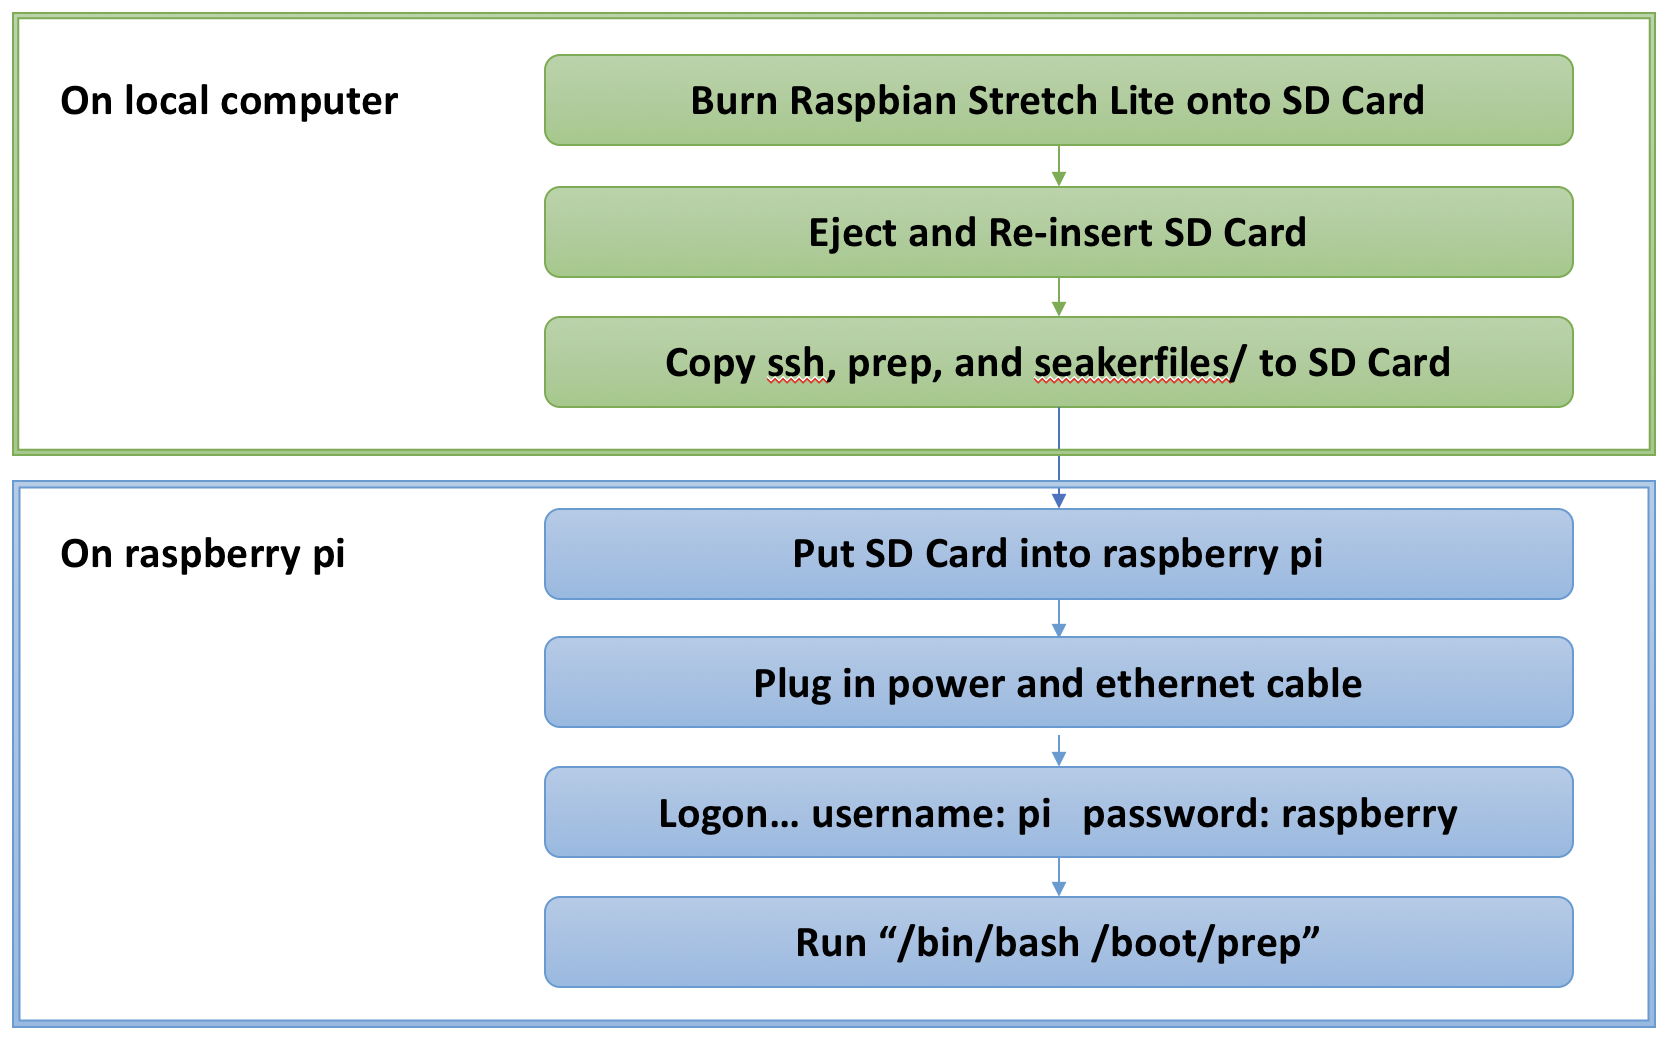
\includegraphics[width=14cm]{images/SeakerCreation.png}
  \caption{SEAKER Creation Process}
  \label{fig:SeakerCreation}
  \end{center}
\end{figure}

\begin{enumerate}
  \item Download the latest Raspbian Stretch Lite operating system\\
  ({\tt https://www.raspberrypi.org/downloads/raspbian/}).
  Note the location where file is saved.
  \item Download the most recent copy of  \verb|prep.sh|, {\tt \gls{ssh}}, and the 
  folder called \verb|seakerfiles|. These files
  contain SEAKER setup and running code.
    \begin{itemize}
      \item \verb|prep.sh| file location: {\tt https://s3-us-west-2.amazonaws.com/seaker/prep.sh}
      \item \verb|ssh| file location: {\tt https://s3-us-west-2.amazonaws.com/seaker/ssh}
      \item \verb|seakerfiles| location: {\tt https://s3-us-west-2.amazonaws.com/seaker/seakerfiles}
    \end{itemize}
  \item Open prep.sh and edit the default configuration information
  (shown below). At minimum it is recommended to change the Raspberry
  Pi and \gls{wifi} passwords.\\

  \lstinputlisting[language=bash]{code/config.sh}

  NOTE: It is recommended to change the \gls{wifi} Name and \gls{ip} Address when
  setting up multiple SEAKER environments over time to ensure each
  environment has unique identifying information.\\
  \\
  For example: If setting up three SEAKER environments, configuration could be:
    \begin{enumerate}
      \item Name: SEAKER01, IP Address: 192.168.101.1
      \item Name: SEAKER02, IP Address: 192.168.102.1
      \item Name: SEAKER03, IP Address: 192.168.103.1
    \end{enumerate}
  \item Insert Micro SD card into computer (not the \gls{rpi}).
  An adapter will likely be required.
  \item Open disk imaging software (Etcher for Mac, or SDFormatter and 
  Win32 Disk Imager for Windows).
  Map to the Raspbian Stretch Lite file
  location, choose the Micro SD card as the destination, and select to burn
  the image. (Refer to the chosen imaging software documentation for
  specific instructions on using this tool.)  Do not remove the micro SD
  card from the computer.
  \item Map to the Micro SD card (Finder for Mac, File Explorer for Windows).
  Copy \verb|ssh|, \verb|prep.sh|, and the \verb|seakerfiles| folder onto the Micro SD card's
  {\em boot} partition.
  \item Remove the Micro SD card from the computer.
  \item Insert the card into the \gls{rpi}.
  \item Power on the \gls{rpi} by plugging it in with the power cord.
  \item Identify the local \gls{ip} Address of the \gls{rpi}:\\
  If installing with Option 1 (router):
    \begin{enumerate}
      \item Plug the \gls{rpi} into the same router being used by the
      Windows or Mac computer.
      \item Use the \gls{ip} Scanning tool on the computer to find the local \gls{ip}
      Address of the \gls{rpi}. The Manufacturer should be ‘Raspberry
      Pi Foundation’.
    \end{enumerate}
  If installing with Option 2 (Direct Connect):
    \begin{enumerate}
      \item Connect the monitor and keyboard to the \gls{rpi}.
      \item Login using the default username (pi) and password (raspberry).
      \item Enter the following command to retrieve the local \gls{ip} Address:\\
      \begin{verbatim}
        ifconfig eth0
      \end{verbatim}
    \end{enumerate}
  If installing with Option 3 (Corporate Network):
    \begin{enumerate}
      \item The MAC Address of the \gls{rpi} is required. This can be
      located on the original \gls{rpi} box.
      \item For Windows systems, open a command prompt and enter the command
      below. Replace the ``c8:26:3b:d2:63:d5'' sequence with the MAC Address
      of the \gls{rpi} being configured.  Use the following command:
      \begin{verbatim}
        arp -a | findstr "c8:26:3b:d2:63:d5"
      \end{verbatim}
      \item For Unix or Linux systems such as Apple or Ubuntu, open a terminal
      window and enter the command below. Replace the ``c8:26:3b:d2:63:d5''
      sequence with the MAC Address of the \gls{rpi} being configured.
      Use the following command:
      \begin{verbatim}
        arp -a | grep "c8:26:3b:d2:63:d5"
      \end{verbatim}
    \end{enumerate}
  \item If installing with Option 1 or 3:
    \begin{itemize}
      \item \gls{ssh} into the \gls{rpi} from the laptop or desktop computer.
      \begin{itemize}
        \item If using a client such as Putty, enter the local \gls{ip} address
        of the \gls{rpi}, choose \gls{ssh} and connect. Click \verb|OK| or
        \verb|Yes| on the security warning.
        \item If using a command line utility such as Bash enter the
        following at the prompt:
        \begin{verbatim}
          ssh pi@<ip_address> -l pi
        \end{verbatim}
        \item Login using the default username (\verb|pi|) and password
        (\verb|raspberry|).
      \end{itemize}
    \end{itemize}
  \item Run the preparation script by typing the following on the command line:
  \begin{verbatim}
    /bin/bash /boot/prep.sh
  \end{verbatim}
  \item Wait for the \gls{rpi} to finish running the script and
  rebooting. The \gls{rpi} should now be configured as a SEAKER
  and be up and running.
\end{enumerate}

\newpage
\subsection{SEAKER Usage}

After collecting all the media devices at the scene, the investigator
will triage them with SEAKER.  Each step of the process is broken
down and discussed in detail below.\\

(1)~Connect the RP to the power and wait for about a minute
to let it finish booting up.
Connect to the RP's Wireless Access Point (\gls{wifi} network). Depending
on the setup, the \gls{wifi}'s SSID will be ``SEAKER01'' or ``SEAKER02''
etc.  See Figure~\ref{fig:screen-1}. Note that SEAKER's Wireless Access
Point is password
protected and matches the one specified in the prep.sh script file.\\

\begin{figure}[ht]
  \begin{center}
  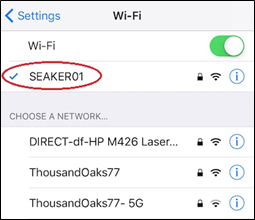
\includegraphics[width=6cm]{images/seaker-hh-screen-1.jpg}
  \caption{iPhone WIFI connection to SEAKER}
  \label{fig:screen-1}
  \end{center}
\end{figure}

(2)~At the same time the investigator may connect all the media
devices to the RP. This may be done concurrently with the previous
step. Note that in order to examine a digital media it will need to be
removed from the
computer, and connected to the RP; this may be done through a
write-blocker interface but it is not necessary.\\

(3)~Once connected to the SEAKER's Wireless Access Point,
the investigator will open any
web browser on their connected device and direct it to go to
{\tt http://seaker01.local}. Access is allowed
through a web browser, as this is the most universal way to connect
on any device (iPhone, iPad, Android, laptop, etc.).  These
devices and many more can connect to a Wireless Access Point
and open a browser.  Once the browser establishes the
connection, the user will see Figure~\ref{fig:screen-2}. Note that the
keywords (or regular expression patterns) present in the ``Type in
Search Terms:'' can be pre-loaded before arriving at the scene, or
changed/updated at the scene.\\

\begin{figure}[H]
  \begin{center}
  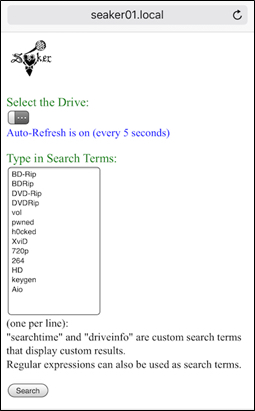
\includegraphics[width=6cm]{images/seaker-hh-screen-2.jpg}
  \caption{Using a browser to connect to {\tt http://seaker01.local}}
  \label{fig:screen-2}
  \end{center}
\end{figure}

The regular expression can be given using the syntax of the
\verb|grep| utility. For example, if we want to find occurrences of
either `two' or `too', we use \verb|t[wo]o|; if we want to find every
word that start with capital letters, we use \verb|^[A-Z]|; if we want
to find words where number~9 is the last character of the line, we use
\verb|9$|. There are a vast number of possibilities; we can also
replace \verb|grep| with \verb|egrep| that has an even richer syntax.\\

(4)~Once any storage media devices that are found at a \gls{searchwarrant} scene
are connected to the RP, the investigator will typically wait for a
few minutes (with some times up to 10 minutes for 1Tb disks with
millions of files) for the file list to be built. Searches can then
be carried out very quickly; essentially, \verb|grep| browses the file
list, line by line, outputting those lines that conform to at least
one pattern specified in the ``Type in Search Terms:'' window. Once
this finishes, the investigator will have the results presented as in
Figure~\ref{fig:screen-3}.

\begin{figure}[H]
  \begin{center}
  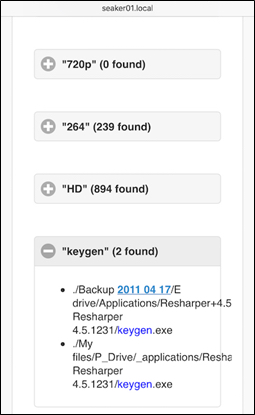
\includegraphics[width=6cm]{images/seaker-hh-screen-3.jpg}
  \caption{The results of the search of a particular device}
  \label{fig:screen-3}
  \end{center}
\end{figure}

The filenames themselves can be incriminating evidence, such as in
Child Pornography (CP) cases, where the material has a commonly used
naming convention, e.g., ``lolita'' which can be found with the \verb|grep|
pattern \verb|.*lolita.*| (`\verb|.*|' means the
following: `\verb|.|' (period)  matches any single character of any
value, except
a newline, and `\verb|*|' (asterisk) matches zero or more of the
preceding character or expression) or simply \verb|lolita|.
This can be used by the
investigators to question the suspects.  The questioning usually
takes place at the same time as the forensic examiners triage the
evidence, and one of the requirements of SEAKER was to be fast so that
investigators can start getting intelligence quickly from the initial
processing of the scene.\\

(5)~The user process flow is documented in the following
figure~\ref{fig:user_process_flow}.

\begin{figure}[ht]
  \begin{center}
  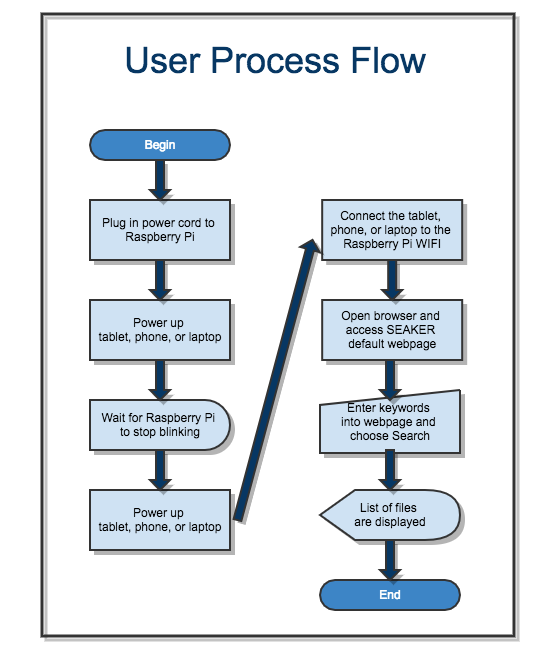
\includegraphics[width=10cm]{images/UserProcessFlow.png}
  \caption{The functionality of SEAKER from the user perspective}
  \label{fig:user_process_flow}
  \end{center}
\end{figure}

\newpage
\subsection{Code}
\subsubsection{Directory and Filename Collection Code (in C)}
\lstinputlisting[language=bash]{code/collect_files.c}

\newpage
\subsection{Results of Testing}
\subsubsection{Collection Timing}

For testing purposes, ls was optimized to utilize as few time-consuming
options as possible, including the {\tt -f} option that prevents sorting
and {\tt -A} for skipping current and parent directories (\verb|.| and
\verb|..|) in the results. Here are the actual functions tested:

\vspace{0.1 cm}
\begin{verbatim}
  sudo sh -c 'cd /mnt/usb && time ls -ARf1 > ~/ls_time.txt'
  sudo sh -c 'cd /mnt/usb && time find / -print > ~/find_time.txt'
  sudo sh -c 'cd /mnt/usb && time ~/collect > ~/collect_time.txt'
\end{verbatim}
\vspace{0.1 cm}

Testing results for the custom collection code vs. operating system file
and directory listing applications:

\begin{center}
  \tiny
    \begin{tabular}{|l|r|r|r|r|r|l|}
    \hline
    \textbf{}                        & \multicolumn{1}{l|}{\textbf{SSD}} & \multicolumn{1}{l|}{\textbf{SSD}} & \multicolumn{1}{l|}{\textbf{\begin{tabular}[c]{@{}l@{}}WD 2.5'\\ SATA HDD\end{tabular}}} & \multicolumn{1}{l|}{\textbf{\begin{tabular}[c]{@{}l@{}}iOmega 3.5'\\ IDE HDD\end{tabular}}} & \multicolumn{1}{l|}{\textbf{\begin{tabular}[c]{@{}l@{}}Samsung 3.5'\\ SATA HDD\end{tabular}}} & \textbf{}                          \\ \hline
    \textbf{Size GB}                 & 500                               & 500                               & 500                                                                                      & 1000                                                                                        & 1000                                                                                          &                                    \\ \hline
    \textbf{Consumed GB}             & 94.22                             & 239.83                            & 456                                                                                      & 474.2                                                                                       & 316.6                                                                                         &                                    \\ \hline
    \textbf{\% Consumed}             & 18.84\%                           & 47.97\%                           & 91.20\%                                                                                  & 47.42\%                                                                                     & 31.66\%                                                                                       &                                    \\ \hline
    \textbf{\# files}                & 1,244,699                         & 1,561,132                         & 14,487                                                                                   & 216,356                                                                                     & 21,556                                                                                        &                                    \\ \hline
    \textbf{\# directories}          & 254,473                           & 317,876                           & 145                                                                                      & 10,603                                                                                      & 2,222                                                                                         &                                    \\ \hline
    \textbf{ls t1}                   & 62.142                            & 112.627                           & 0.942                                                                                    & 8.398                                                                                       & 1.400                                                                                         &                                    \\ \hline
    \textbf{ls t2}                   & 62.025                            & 116.978                           & 0.899                                                                                    & 8.252                                                                                       & 1.375                                                                                         &                                    \\ \hline
    \textbf{ls t3}                   & 68.376                            & 115.833                           & 0.903                                                                                    & 8.229                                                                                       & 1.324                                                                                         &                                    \\ \hline
    \textbf{ls ave time (secs)}      & \textbf{64.181}                   & \textbf{115.146}                  & \textbf{0.915}                                                                           & \textbf{8.293}                                                                              & \textbf{1.366}                                                                                & \textbf{}                          \\ \hline
    \textbf{find t1}                 & 43.914                            & 90.693                            & 1.004                                                                                    & 9.090                                                                                       & 1.733                                                                                         &                                    \\ \hline
    \textbf{find t2}                 & 44.958                            & 97.619                            & 1.014                                                                                    & 8.315                                                                                       & 1.667                                                                                         &                                    \\ \hline
    \textbf{find t2}                 & 43.214                            & 96.499                            & 1.015                                                                                    & 8.347                                                                                       & 1.672                                                                                         &                                    \\ \hline
    \textbf{find ave time (secs)}    & \textbf{44.029}                   & \textbf{94.937}                   & \textbf{1.011}                                                                           & \textbf{8.584}                                                                              & \textbf{1.691}                                                                                & \textbf{}                          \\ \hline
    \textbf{col t1}                  & 20.893                            & 68.270                            & 0.834                                                                                    & 7.541                                                                                       & 1.281                                                                                         &                                    \\ \hline
    \textbf{col t2}                  & 18.103                            & 82.091                            & 0.832                                                                                    & 7.548                                                                                       & 1.260                                                                                         &                                    \\ \hline
    \textbf{col t3}                  & 19.381                            & 84.823                            & 0.804                                                                                    & 7.531                                                                                       & 1.248                                                                                         &                                    \\ \hline
    \textbf{collect ave time (secs)} & \textbf{19.459}                   & \textbf{78.395}                   & \textbf{0.823}                                                                           & \textbf{7.540}                                                                              & \textbf{1.263}                                                                                & \textbf{Average:}                  \\ \hline
    \textbf{\% faster than ls}       & 70\%                              & 32\%                              & 10\%                                                                                     & 9\%                                                                                         & 8\%                                                                                           & \multicolumn{1}{r|}{\textbf{26\%}} \\ \hline
    \textbf{\% faster than find}     & 56\%                              & 17\%                              & 19\%                                                                                     & 12\%                                                                                        & 25\%                                                                                          & \multicolumn{1}{r|}{\textbf{26\%}} \\ \hline
    \end{tabular}
  \captionof{table}{Collection Algorithm Timing Data}
  \label{tab:CollectionAlgorithmData}
\end{center}

TODO: add more result data\\

\newpage
\bibliographystyle{plain}
\bibliography{references}

\end{document}

